\documentclass[11pt]{article}
\usepackage[ngerman]{babel}
\usepackage{graphicx}
\usepackage[export]{adjustbox}
\usepackage[acronym]{glossaries}
\usepackage[backend=biber, style=apa]{biblatex}
\usepackage{geometry}
\usepackage{fontspec}
\usepackage{float}
\usepackage{titlesec}
\usepackage{hyperref}

\titleformat{\section}
  {\normalfont\fontsize{12}{15}\bfseries}{\thesection}{1em}{}

\titleformat{\subsection}
  {\normalfont\fontsize{12}{15}\bfseries}{\thesubsection}{1em}{}

\titleformat{\subsubsection}
  {\normalfont\fontsize{12}{15}\bfseries}{\thesubsubsection}{1em}{}


\setmainfont{Arial}
    \geometry{margin=2cm}

    \DeclareLanguageMapping{german}{german-apa}
    \addbibresource{references.bib}

    \author{Benedikt Magnus Hering}
    \title{IPWA02 - Projektdokumentation}
    \date{27. Oktober 2023}

    \newpage

    
    \makenoidxglossaries
    \newacronym{javaee}{Java EE}{Java Enterprise Edition}
    \newacronym{jakartaee}{Jakarta EE}{Jakarta Enterprise Edition}
    \newacronym{jsf}{Jsf}{JavaServer Faces}
    \newacronym{beans}{Beans}{Enterprise JavaBeans}
    \newacronym{hibernate}{Hibernate}{Hibernate ORM}
    \newacronym{css}{Css}{Cascading-Style-Sheets}
    \newacronym{daos}{Daos}{Data-Access-Objects}
    \newacronym{regex}{Regex}{Regular Expression}
    \newacronym{uml}{Uml}{Unified Modeling Language}


    \begin{document}

    \begin{titlepage}
        \begin{center}
            
\includegraphics[max width=\textwidth]{iu_logo.png}
            \textbf{Projektdokumentation}
            \\[1\baselineskip]
            IPWA02-01 - Programmierung von industriellen Informationssystemen mit Java EE
            \\[1\baselineskip]
            Studierender: Benedikt Magnus Hering
            \\
            Matrikelnummer: 92011026 
            \\
            Studiengang: B.Sc. Softwareentwicklung
            \\
            GitHub-Repository: \href{https://github.com/Herry3108/ipwa02}{https://github.com/Herry3108/ipwa02}
            \\[1\baselineskip]
            Modulverantwortlicher: Herr Prof. Dr. Marian Benner-Wickner
            \\
            Tutor: Herr Paul Libbrecht
            \\[2\baselineskip]
            Abgabedatum: 09.12.2023, Stuttgart
        \end{center}    
    \end{titlepage}

    \pagenumbering{Roman}

    \tableofcontents

    \newpage
    \listoffigures
    \addcontentsline{toc}{section}{Abbildungsverzeichnis}

    \newpage
    \printnoidxglossaries
    \addcontentsline{toc}{section}{Akronyme}

    \newpage
    \pagenumbering{arabic}
    \section{Einleitung}
    Die folgende Projektdokumentation bezieht sich auf die Bearbeitung der Aufgabenstellung 1.3 des Moduls 
    IPWA02-01 - Programmierung von industriellen Informationssystemen mit Java EE
    an der Hochschule IU - Internationale Hochschule. 
    Innerhalb des Skrips wurde die Technologie Java EE gelehrt, welche innerhalb der Projektarbeit verwendet wird.
    Um der Weiterentwicklung von Java EE gerecht zu werden, wird das Wording \gls{jakartaee} verwendet. Die Namesänderung ist auf die Rechteübertragung
    der Java EE Entwicklung von Oracle zur Eclipse Foundation zurückzuführen. 
    (\cite{jakarta_ee})
    Bei der Verwendung von Jakarta EE wird ein großer Fokus auf die Nutzung von 
    \gls{jsf},
    \gls{beans},
    \gls{hibernate} 
    und Primefaces gelegt.

    \subsection{Fallstudie und Zielsetzung}
    Durch die Aufgabenstellung wird der Rahmen vorgegeben, dass eine Webapplikation für eine Non-Profit-Organisation namens „Shea Sepherd“ zu erstellen ist. 
    Die Organisation möchte eine Website erstellen, die sich auf die Meldung und Bergung von verschollenen Fischernetzen fokussiert. Da explizit auf die Entwicklung eines Prototyps hingewiesen ist,
    wird darauf auch der Fokus gelegt. Es wird ein grundlegendes Designkonzept für die Website erstellt, jedoch das Hauptaugenmerk
    auf die technische Umsetzung und Programmierung gelegt.  

    \subsection{Verlaufsplanung}
    Zu Beginn des Projektes wird ein Designkonzept, durch die Verwendung des agilen Frameworks des Design-Thinkings erstellt.
    Anschließend beginnt der Entwicklungsprozess, der sich in acht Teilschritte unterteilt. Um ein strukturiertes Vorgehen während der
    Programmierung zu gewährleisten, wird mit der Erstellung der \gls{uml}-Diagramme für die Beans, Controller, \gls{daos} und Entitäten begonnen. Anschließend wird die
    Entwicklungsumgebung, IntelliJ IDEA, für den kommenden Entwicklungsprozess vorbereitet. Sobald die Vorbereitung dessen abgeschlossen ist, wird die Datenbank
    erstellt. Nach Abschluss des vorherigen Schrittes wird die Datenbankinstanz mit der Entwicklungsumgebung, durch Verwendung von Hibernate und Jakarta-Persistence, verknüpft und die benötigten Relationstabellen erstellt. Der vierte Schritt des Entwicklungsprozesses ist die Erstellung der
    Entitäten, welche die zuvor erstellten Tabellen in Form von Java-Dateien nachbilden. Um den Zugriff auf die Entitäten zu steuern, werden Datenbankzugriffsobjekte verwendet.
    Diese Objekte beinhalten die verschiedenen Zugriffsmethoden auf die Relationen, durch Verwendung der Entiäten. Um die Datenverwaltung der jeweiligen Seite abzudecken, werden die sogennanten Beans verwendet. Beans sind für
    die Datenhaltung zuständig. Um ebenfalls Methoden, welche über die ledigliche Datenhaltung hinaus gehen, abzudecken, werden Controller verwendet. Durch Controller werden beispielsweise Schnittstellenabrufe getätigt. 
    Durch das Abschließen der vorherigen Schritte ist die Datenbank und das Backend erstellt. Im kommenden Schritt wird die Implementierung des Frontends am Beispiel der Verwaltungsseite getätigt. Innerhalb dieses Schrittes
    wird die Frontend-Technologie Primefaces eingesetzt.
    \\
    Nach Beendigung der Programmierung ist es wichtig, die Webapplikation ausreichend zu testen, um dem Endnutzer eine fehlerfreie Nutzung zu gewährleisten.
    Um dieses Qualitätsziel zu erfüllen, wird die Webapplikation anhand von Funktionstest geprüft und Fehler dokumentiert. Sollten Fehler vorhanden sein, werden diese
    anschließend behoben.
    \\
    Danach wird die fertig erstellte Software innerhalb eines GitHub-Repository veröffentlicht.
    \\
    Als letzter Schritt wird der Verlauf des Projekts analysiert und sowohl gute, als auch schlechte Punkte hevorgehoben.

    \newpage


    \section{Hauptteil}
    Im ersten Schritt des Projekts sind aus sieben vorhanden Aufgaben, fünf zu priorisieren. Die Aufgaben sind bereits anhand der MoSCoW-Methode priorisiert, welche 
    diese nach deren Priorität in Must, Should, Could und Won't unterteilt. Jede diese vier Kategorien stellt die Wichtigkeit der jeweiligen Aufgabe für den Erfolg des Projekts dar.
    Im zugrundeliegenden Fall sind vier Unteraufgaben mit Must und drei mit Should markiert. Da die Aufgaben
    mit der Priorisierung Must die höchste Wichtigkeit aufweisen, sind alle dieser vier Aufgaben in der Umsetzung zu berücksichtigen.
    Hierbei handelt es sich um die Erfassung von Geisternetzen als meldende oder anonyme Person, der Eintragung 
    als bergende Person zur Geisternetzbergung, einer Übersicht der noch zu bergenden Geisternetze als bergende Person und
    der Möglichkeit als bergende Person Geisternetze als geborgen melden zu können. 
    Als fünfte Unteraufgabe wird die Funktion gewählt, als anonyme Person Geisternetze verschollen melden zu können.

    \subsection{Design-Thinking}
    Um das Designkonzept der Webapplikation zu entwickeln, wird das Framework des Design-Thinkings verwendet.
    Es wird das Ziel verfolgt, sich ein Design anhand eines tiefgreifenden Wissens, passend zur Thematik zu 
    erschließen. Begonnen wird mit dem ersten Schritt des Verstehens. Hierbei wird sich mehr in die Rolle
    des Protagonisten, dem Webentwickler der Non-Profit-Organisation, hinein versetzt. Es ist von Wichtigkeit zu verstehen, was die Beweggründe und
    Absichten der Person sind. Der zweite Schritt namens Beobachtung, beschäftigt sich tiefgreifender mit den Hintergründen der Thematik.
    Anhand von Fakten und Daten wird ein größeres Verständnis zur Thematik entwickelt. Anschließend kommt der dritte Schritt, welcher sich mit dem Verständnis
    der Sichtweisen beschäftigt. Hierbei wird eine Relation zwischen dem ersten und dem zweiten Schritt hergestellt, um eine fundierte Grundlage für die weiteren Schritte zu definieren. Im vierten Schritt werden Ideen für die Umsetzung der Website entwickelt. 
    Begonnen wird mit der Phase des Brainstormings, welche den Gedanken freien Lauf lässt. Danach werden diese anhand von verschiedenen Faktoren bewertet und anschließend priorisiert.
    Folgend wird ein Prototyp entwickelt, welcher die zuvor erstellten Denkansätze in die Tat umsetzt. Zuletzt wird der Prototyp dem Kunden vorgestellt und dessen Feedback eingeholt.

    \subsubsection{Verstehen - Das Problem definieren}
    Im ersten Schritt des Design-Thinkings ist es wichtig, sich ein solides Fundament zu schaffen.
    Eine solide Ausgangssituation zeichnet sich durch ein zu lösendes Problem aus Sicht des Kunden / Unternehmen und einer transparent vorgegebenen Rahmenbedingungen zur Erfüllung
    des Problems aus. (\cite{design_thinking})
    In der Ausgangssituation ist dies durch die Aufgabenstellung bereits großteils vorhanden. 
    Bisher besteht lediglich das Fachkonzept des Requirements Engineers, dass Anforderungen an die zu erstellende Webapplikation vorgibt.
    Die Problematik aus Sicht des Webentwicklers ist es, die bisherigen Anforderungen in einer Webapplikation zu verwirklichen. Dazu muss sowohl ein Designkonzept, 
    als auch eine Softwarearchitektur erstellt werden. Anschließend gilt es dies durch die Programmierung umzusetzen. 
  
    \subsubsection{Beobachten - Kundenbedürfnisse verstehen}
    Das Beobachten zum Verstehen der Kundenbedürfnisse, ist in diesem Fall auf den eigenen Arbeitgeber und dessen Kunden Zielgruppen begrenzt.
    Um die Gefahrenlage von Geisternetzen für die Meeresbewohner und Natur besser zu verstehen, müssen die problematischen Auswirkungen von 
    Geisternetzen näher betrachtet werden.
    Geisternetze stellen für mehr als 344 Tierarten eine potenzielle Gefahr da. Vor allem sind hiervon Meeresbewohner, Schildkröten
    und Seevögel betroffen. Diese können sich beispielsweise in herrenlosen Netzen verfangen und dadurch Ertrinken, da diese keinen
    Sauerstoff mehr aufnehmen können. Des Weiteren droht die Gefahr, dass sich die Netze langsam zersetzen und somit
    eine Belastung durch Mikroplastik freisetzen. Dieses Mikroplastik kann durch die Nahrung der Tiere mit aufgenommen werden
    und für diese im schlimmsten Falle zum Tod führen. (\cite{wwf_geisternetz})
    Um diesen problematischen Zustand entgegenzuwirken, müssen Maßnahmen getroffen werden.

    \subsubsection{Standpunkt definieren - Was haben wir gelernt?}
    „Dein Ziel ist es, auf Basis der gesammelten Annahmen und Beobachtungen einen konzeptionellen Rahmen zu entwickeln, der den Lösungsraum absteckt und der deinen idealen Kunden definiert.“ (\cite{design_thinking})
    \\[1\baselineskip]
    Angelehnt an das obige Zitat von Andreas Diehl ist die in den ersten beiden Schritten erarbeitete Wissensbasis zu verfeinern. Es ist sowohl die Problematik aus Sicht des Webentwicklers bekannt,
    als auch ein tiefgreifenderes Verständnis der Sichtweise der Non-Profit-Organisation geschaffen.
    Die Beweggründe der Organisation „Shea Sepherd“ und deren Mitarbeitern, sind durch deren geschäftlichen Kontext einzuordnen und fokussieren
    sich auf den Schutz der Umwelt und Tiere.
    Ableiten lässt sich daraus ein umweltbewusster Endnutzer der Webapplikation. Dessen Ziele sind es, die durch die Geisternetze ausgehende Gefahrenlage zu minimieren und auf die Notwendigkeit von dessen Bergung aufmerksam zu machen. 

    \subsubsection{Ideen entwickeln - Lösungen skizzieren und priorisieren}
    Eine einfache und selbsterklärende Bedienung der Web-Applikation sollte gegeben sein, da der Fokus auf der Koordinierung zur Bergung und Meldung der Netze liegt.
    Innerhalb dieses Schritts, wird sich mit der Ideenentwicklung beschäftigt. Selbst wird dieser in drei weitere Schritte unterteilt, 
    die sich in Sammlung, Bewertung und Priorisierung gliedern.
    \\[1\baselineskip]
    Beginnend mit dem ersten Teilschritt namens Sammlung, wird den Gedanken durch ein Brainstorming freier Lauf gelassen.
    Zuerst ist festzulegen, wie die Nutzererkennung auf der Webapplikation verwirklicht wird.
    Einerseits wäre die Steuerung der aktiven Nutzer über ein Login-Formular möglich. Jede Person, welche Meldungen erfassen oder Bergungen vornehmen möchte, 
    muss sich auf der Website registrieren. Um jedoch die Möglichkeit, der anonymen Meldung von Geisternetzen, zu gewährleisten, kann eine Person sich auch über einen Button namens
    „Anonym fortfahren“ auf der Website anmelden oder diese lediglich aufrufen.
    \\
    Das Gegenstück wäre eine Webapplikation, welche ohne Login-Formular und Speicherung der Nutzerdaten, die Meldung von Geisternetzen zulässt.
    So kann jede Person Geisternetze melden, ob anonym oder persönlich. Eine Registrierung auf der Website kann vorgenommen werden, ist jedoch optional. Die Meldung der Geisternetze ist sowohl persönlich, durch eine Registrierung auf der Website möglich,
    als auch anonym durch das direkte Aufrufen. Um Geisternetze hingegen bergen zu können, ist eine
    Registrierung auf der Website zwingend erforderlich. Der Nutzer kann bei seiner Registrierung festlegen, ob er eine meldende und / oder bergende
    Person sein möchte.
    Nachdem die Ideensammlung zur Nutzererfassung vollendet ist, wird der Hauptbereich der Website durchdacht.
    Eine Möglichkeit wäre der Aufbau über eine große interaktive Weltkarte. Der Endnutzer muss lediglich auf den Standort des Geisternetzes klicken, um die Meldung zu erstellen.
    Des Weiteren kann diese Karte auch zur Koordinierung und Zuweisung der Bergungen dienen. 
    Die auf der Weltkarte erfassten Meldungen werden in unterschiedlichen Farben angezeigt. So könnte beispielsweise die Farbe rot für noch offene, gelb für bereits zugewiesene und grün für abgeschlossene
    Bergungen gelten. Möchte der bergende Nutzer sich eine offene Meldung selbst zuweisen, orientiert er sich anhand der roten Markierungen und kann diese per Klick beanspruchen. 
    \\
    Konträr wäre die Erfassung der Geisternetzmeldungen über ein klassisches Formular steuerbar. Für jeden wichtigen
    Wert, welcher für die Meldung des eines Geisternetzes nötig ist, gibt es ein eigenes Formularfeld. Die Speicherung
    der Meldung wird über einen Speichern-Button gesteuert. Anschließend werden verschiedenen Tabellen für
    die Übersicht nach offenen, selbst zugewiesenen und verschollen Bergungen genutzt. Innerhalb dieser Tabellen sind
    Checkboxen für die jeweilige Aktion hinterlegt, welche eine schnelle Steuerung des aktuellen Zustands des Geisternetzes
    bieten. 
    \\
    Nach Abschluss der Phase des Brainstormings, werden die Ergebnisse bewertet. Die Bewertung sollte vor allem die Priorität auf 
    die Vereinbarkeit von Wirtschaftlichkeit, Machbarkeit und Erwünschtheit legen.(\cite{design_thinking})
    Um die Wirtschaftlichkeit des jeweiligen Umsetzungsvorhabens zu messen, wird der dafür nötigen Zeitaufwand gemessen.
    Die erste Gegenüberstellung ist die verpflichtende und die optionale Nutzererkennung.
    Die verpflichtende Variante ist kostengünstiger. Dies lässt sich anhand der Komplexität der Implementierung
    zeigen, da es lediglich eine einzelne Implementierung ist. Während das
    optionale Einloggen sowohl die Implementierung des Login-Formulars, als auch die Nutzung der Website
    ohne diese beinhaltet, woraus zwei Implementierungen resultieren.
    \\
    Anschließend folgt die Gegenüberstellung der interaktive, Weltkarte, zur Formular und Tabellen getriebenen Variante.
    Einerseits ist die Implementierung einer interaktiven Weltkarte ist für den Nutzer ein einzigartiges Erlebnis. 
    Das Alleinstellungsmerkmal ist, dass dem Nutzer selten eine solche User-Experience geboten wird. Die Implementierung einer interaktiven Weltkarte
    ist jedoch mit einem hohen Zeitaufwand verbunden, da kaum auf bereits bestehende Technologie-Bibliotheken zurückgegriffen werden kann. Es müsste eine Weltkarte eingebunden werden und diese mit verschiedenen Funktionen
    im Vorder- und Hintergrund verknüpft werden.
    Der Kontrahent, des Aufbaus durch Formular- und Tabellenansichten, bietet hingegen einen weit verbreiteten Standard des Website-Aufbaus. Aus diesem Grund
    ist dieser Aufbau die kostengünstigere Variante. Die meisten Websites sind mit Formularfeldern und Tabellen versehen, 
    weshalb die Verwendung einer der vielen verschiedenen \gls{css}- und JavaScript-Bibliotheken den Aufwand zur Implementierung drastisch verringern kann.
    \\
    Im letzten Schritt gilt es die erarbeiteten und bewerteten Ideen zu priorisieren.
    Als Erstes ist die Art des User-Logins zu betrachten. Da aufgrund der Aufgabenstellung
    ebenfalls eine anonyme Meldung von Geisternetzen möglich sein soll, ist hierbei das optionale Login zielführender.
    Jede Person kann schnell und einfach ein gesichtetes Geisternetz melden. Durch das nicht zwingende
    Anmelden auf der Website ist die Bedienung für den Endnutzer einfacher und intuitiver.
    Bei der Entscheidung zwischen der interaktiven Weltkarte und der klassischen Steuerung der Website, ist letzteres für die Aufgabenstellung zielführender.
    Die zu erstellenden Website ist im Rahmen einer Hausarbeit eines Hochschulprojekts umzusetzen,
    weshalb dessen Komplexität nicht künstlich verstärkt werden soll. Aus diesem Grund wird der tabellarische und formulargetriebe Aufbau der Website gewählt.
    
    \newpage
    \subsubsection{Prototyping - Modellierung der besten Idee}
    Das Prototyping des Designs wird über das Design-Tool Figma erstellt. Letzteres bietet die Möglichkeit
    über eine Webapplikation einen interaktive Prototypen zu erstellen.
    \begin{figure}[H]
        \centering
        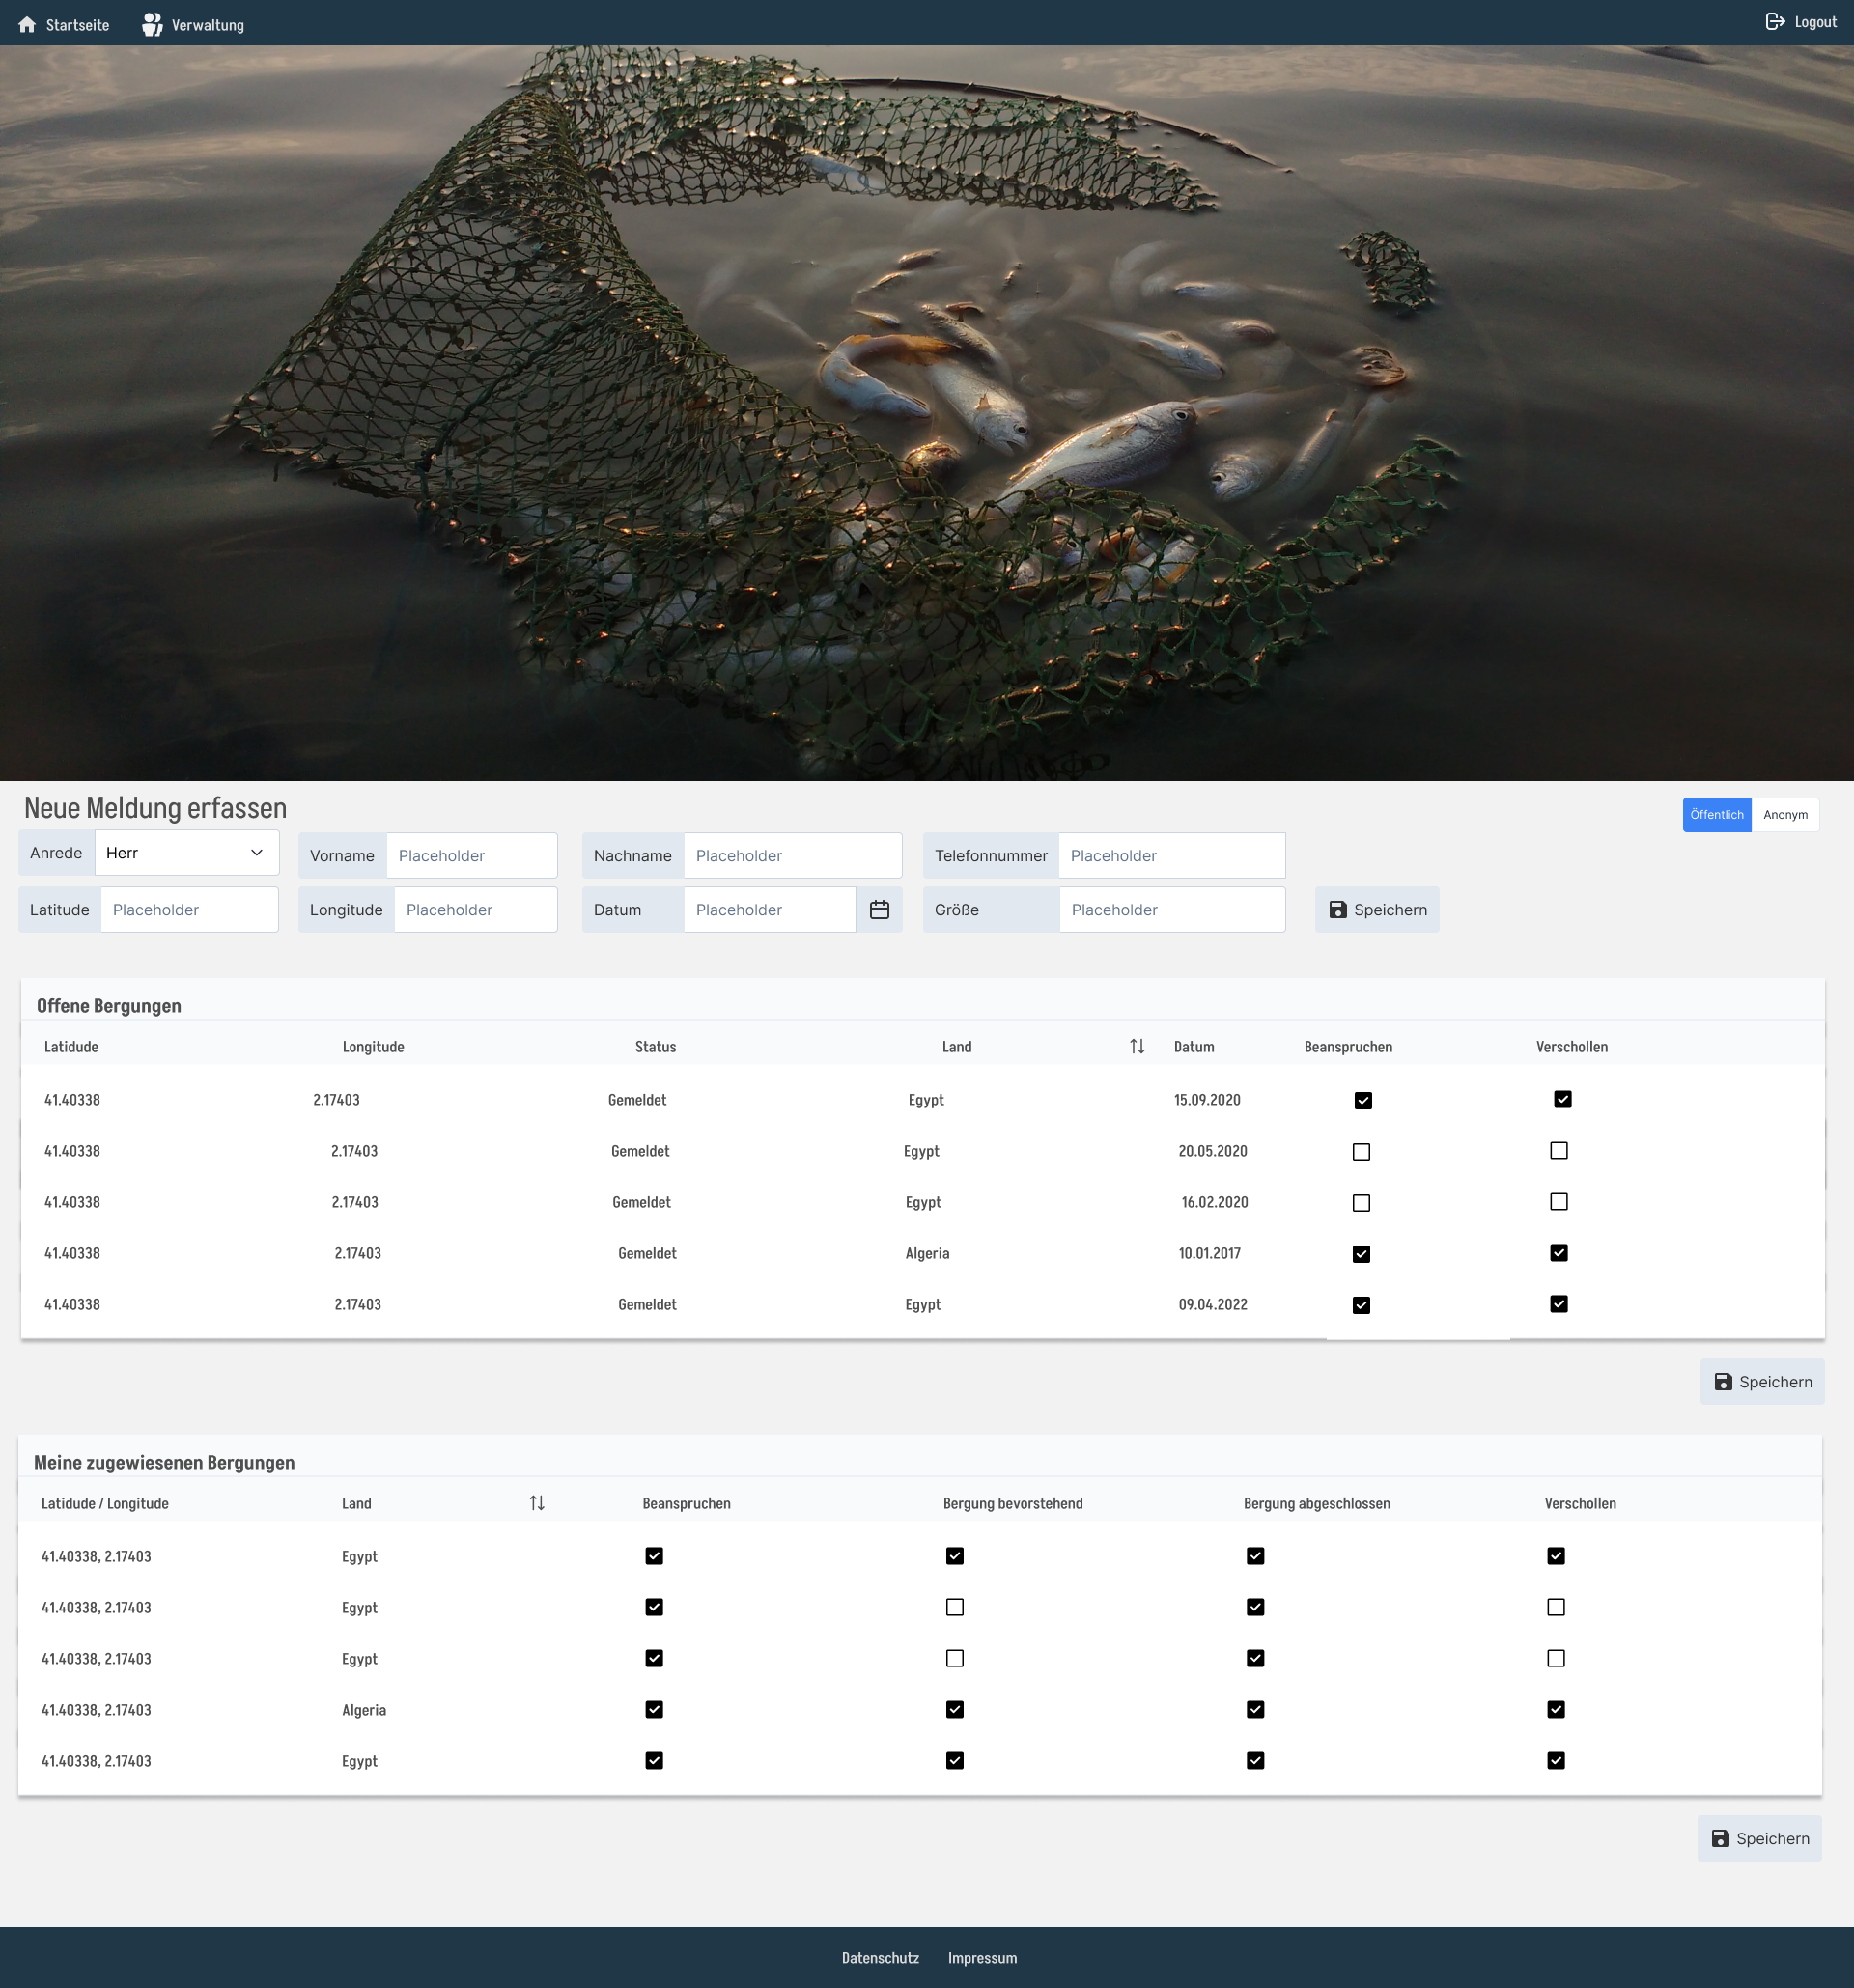
\includegraphics[width=\textwidth]{abbildungen/Verwaltungsseite.png}
        \caption{Design der Verwaltungsseite in Figma}
        \label{verwaltung-figma}
    \end{figure}

    \newpage
    Eine beispielhafte Erarbeitung eines Prototyps wird folgend anhand der Verwaltungsseite demonstriert.
    Innerhalb der Verwaltungsseite soll die Meldung und Bergung von Geisternetzen koordiniert werden.
    Um dies für den Nutzer einfach und intuitiv zu gestalten, wird der Hauptbereich dieser Seite in drei Bereiche unterteilt. Der erste Bereich gilt für
    die Erstellung neuer Meldungen durch ein Formular. Das Formular besitzt an der oberen rechten Ecke einen Schalter, der zwischen der persönlichen
    und anonymen Meldung von Geisternetzes unterscheidet. Hat der Schalter den Zustand persönlich,
    so ist die erste Reihe des Formulars für die Eingabe der Nutzerdaten vorhanden. Der Nutzer kann 
    hier seine persönlichen Daten wie Anrede, Vorname und Nachname eingeben. Sollte der Nutzer sich zusätzlich auf der 
    Website eingeloggt haben, so sind dessen Daten vor eingetragen. Ist hingegen eine anonyme Meldung gewünscht, so ist die erste Reihe des Formulars
    deaktiviert. Die zweite Reihe des Formulars dient zur Erfassung der Eigenschaften des Geisternetzes. Hierfür sind die Latitude, Longitude, Erfassungsdatum
    und die Größe des Geisternetzes zu hinterlegen. Rechts unterhalb des Formulars ist ein Button zur Speicherung der Formulardaten hinterlegt.
    \\
    Der zweite Bereich der Website stellt eine Tabelle der aktuellen offenen Bergungen zur Übersicht dar. 
    Sollte ein aktiver bergender Nutzer auf der Webapplikation 
    eingeloggt sein, so ist eine zusätzliche Spalte namens „Beanspruchen“ mit Checkboxen verfügbar. Durch die Aktivierung einer Checkbox, weist sich der 
    Endnutzer eine offene Meldung zu. Ist hingegen keine oder eine lediglich meldende Person eingeloggt, ist letztere Spalte der Tabelle deaktiviert. In jedem Fall ist für den Endnutzer 
    eine Spalte zum Verschollen melden der jeweiligen Meldung vorhanden.
    Sollten verschollene Meldungen vorhanden sein, werden diese unterhalb in einer eigenständigen Tabelle angezeigt.
    \\
    Zuletzt ist für eingeloggte bergende Nutzer eine Tabelle sichtbar, welche eine Übersicht über die 
    selbst zugewiesenen Bergungen gibt. Wie gewohnt sind die wichtigsten Informationen des jeweiligen Geisternetzes hinterlegt. Die Steuerung der Geisternetzzuweisungen ist über die Beanspruchen-Spalte möglich. Hier kann der Nutzer seine Zuweisung zum 
    Geisternetz durch einen Klick wieder aufheben. Um die Möglichkeit zu bieten, den Status der Geisternetze selbst zu aktualisieren, sind die letzten drei Spalten der Tabelle mit Checkboxen versehen. Diese sind zur Steuerung der Status „Bergung bevorstehend“,
    „Bergung abgeschlossen“ und „Verschollen„“ zuständig.

    \newpage
    \subsubsection{Testen - Was sagt der Kunde?}
    Nachdem das Designkonzept als Prototyp modelliert wurde, ist dies auf die Zufriedenheit des Kunden zu testen.
    Da diese Fallstudie sich in einer fiktiven Umgebung befindet, wird die Zufriedenheit des Kunden als Synonym zu einer einfachen und selbsterklärenden Website gesehen.
    Da das Design des Prototyps sich an den gängigen Aufbau einer Website hält, befindet sich der Endnutzer
    in einer gewohnten Umgebung. Die simple Bedienung der Webapplikation, durch Formulare und Tabellen, bietet dem 
    Endnutzer eine bereits bekannte und selbsterklärende Erfahrung. Daraus resultierend ist die Zufriedenheit des Kunden erfüllt.

    \newpage
    \subsection{Entwicklungsprozess}
    Der folgende Abschnitt bezieht sich auf die Programmierung der Webapplikation. Da im Studienskript das Java-Framework,
    Jakarta EE, mit Schwerpunkt auf \gls{jsf} und \gls{hibernate}, gelehrt wird, werden diese Technologien für die 
    Programmierung des Backend und der Datenbanken verwendet. Für das Frontend der Website wird das Framework Primefaces verwendet.

    \subsubsection{Erstellung der Uml-Diagramme}
    Um eine strukturierte Programmierung zu gewährleisten, werden vor Beginn der Quellcodeerstellung die Java-Klassen in Uml-Diagrammen modelliert.
    Zur Bildung des Fundaments der Webapplikation, wird mit dem Datenmodell begonnen. Die Datenstruktur wird durch ein Entity-Relationship-Diagramm modelliert.
    \begin{figure}[H]
        \centering
        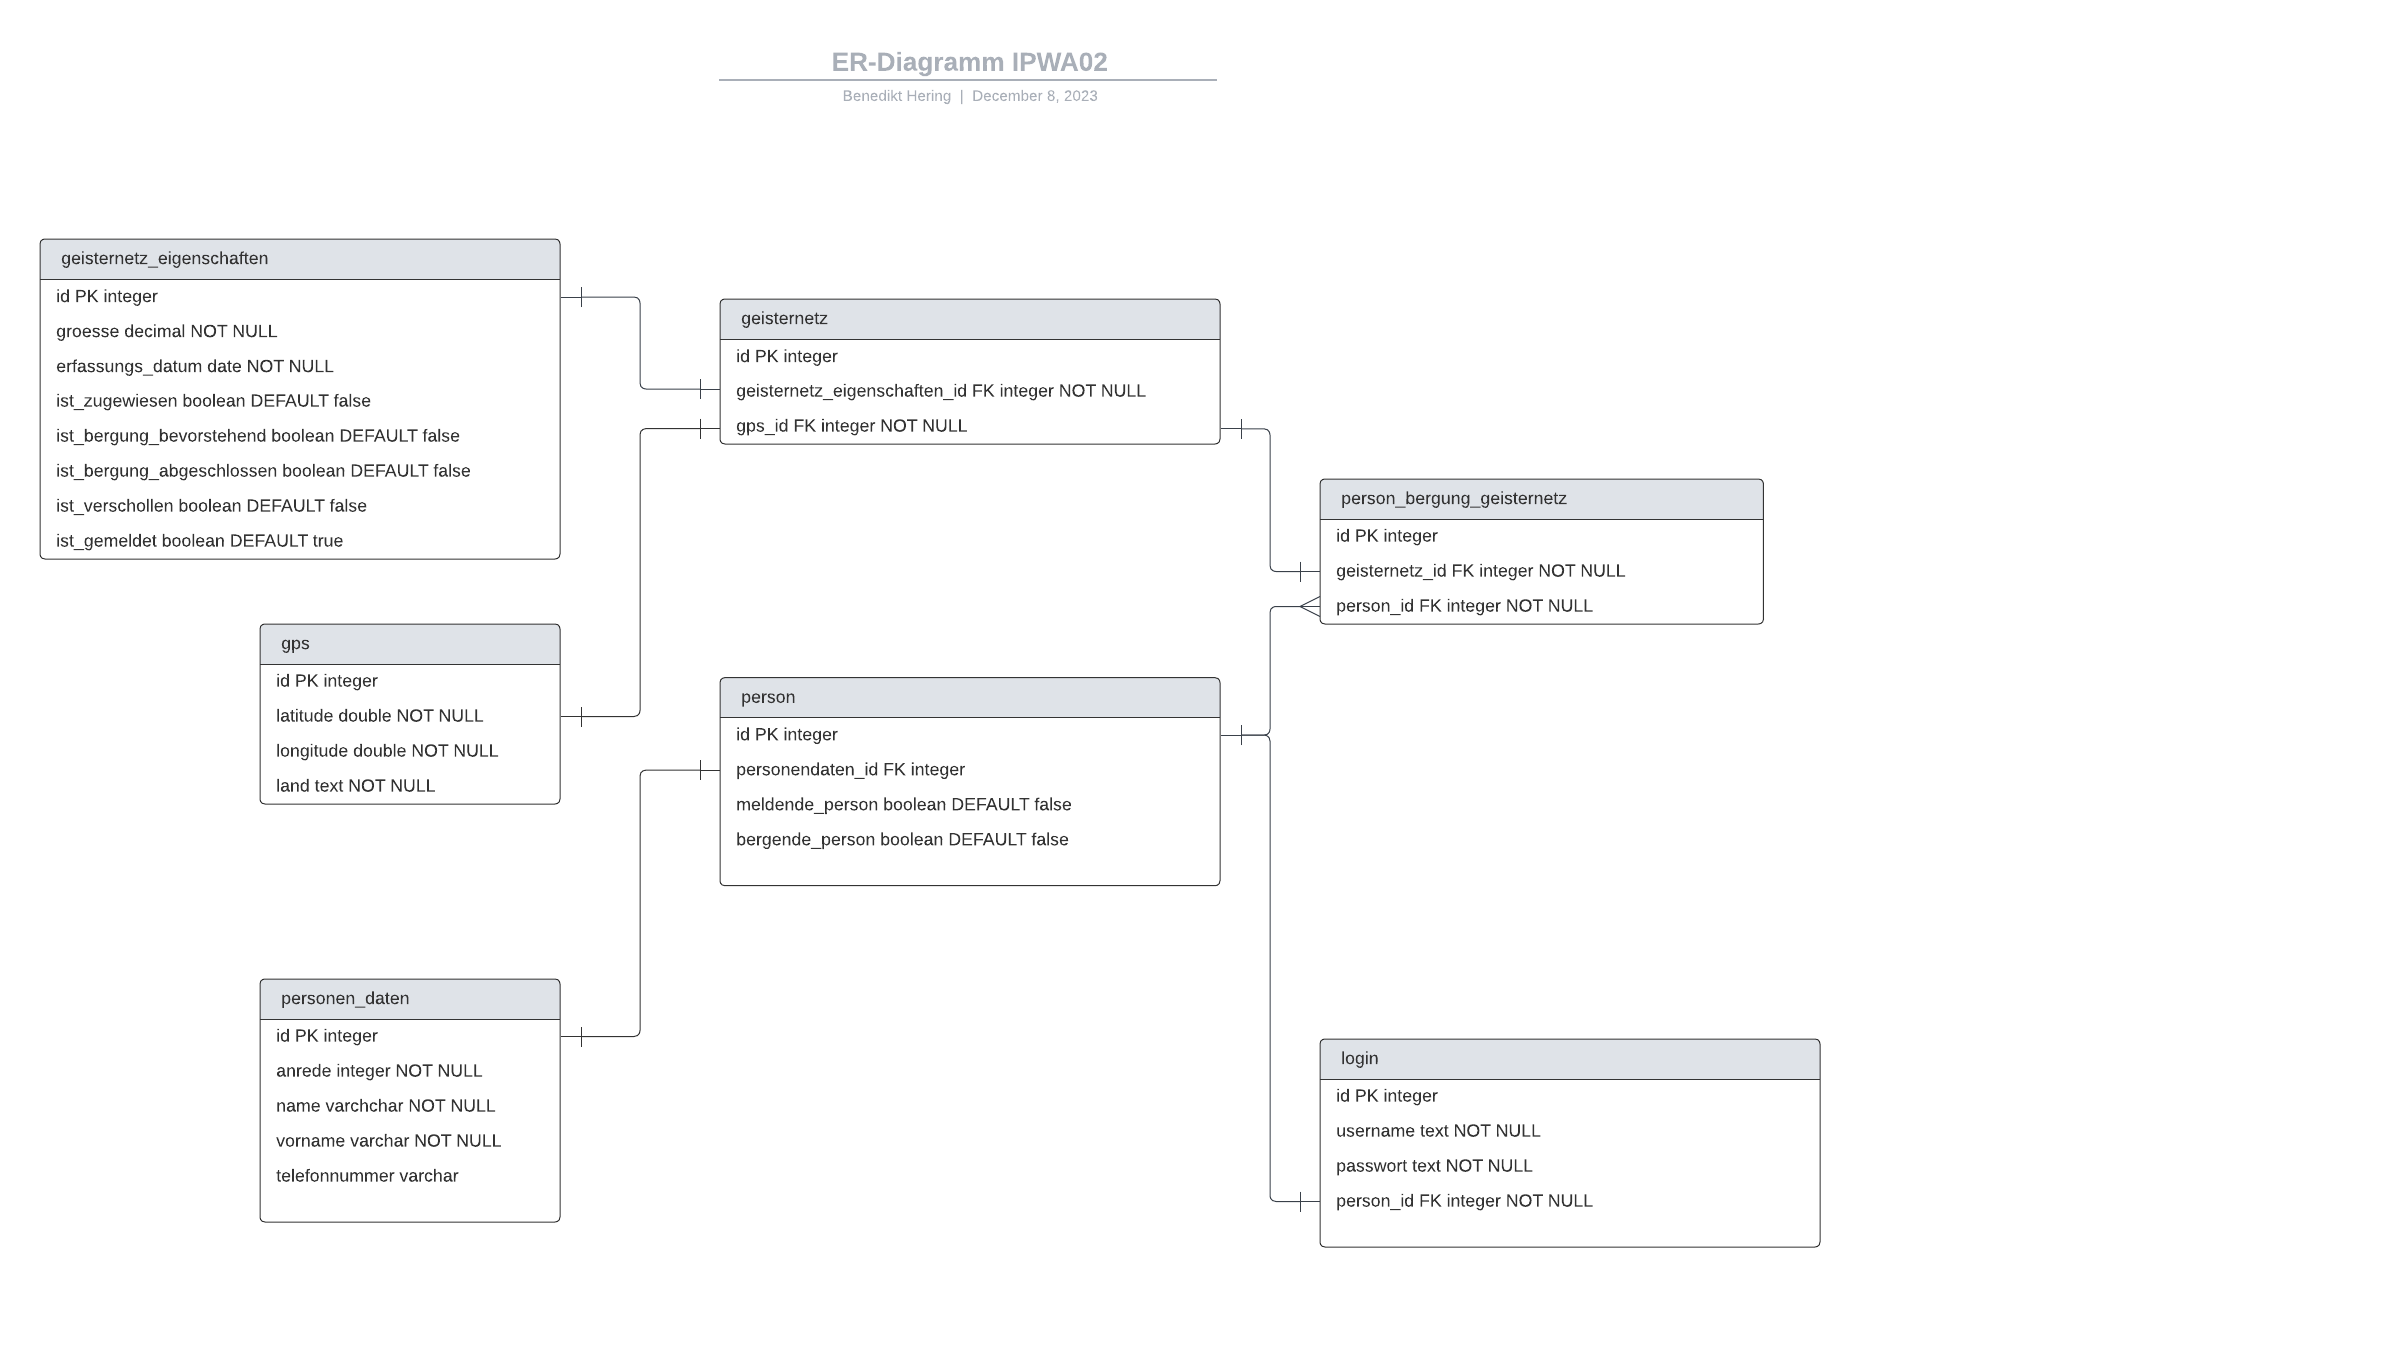
\includegraphics[width=\textwidth]{abbildungen/ER-Diagramm.png}
        \caption{ER-Diagramm}
        \label{er-diagramm}
    \end{figure} 
    Der Datenbankaufbau wird anhand von drei Haupttabellen namens Person, Geisternetz und PersonBergungGeisternetz gebildet.
    Die Tabelle Person dient zur Verwaltung der meldenden und bergenden Personen. Innerhalb der Tabelle Person selbst, ist 
    eine Fremdschlüssel-Relation zur Tabelle PersonenDaten hinterlegt, welche die persönlichen Daten der Personen
    verwaltet. Des Weiteren sind zwei Spalten namens „ist\_meldend“ und „ist\_bergend“ hinterlegt, welche die Rechte der jeweiligen Person abbilden.
    Die zweite Haupttabelle namens Geisternetz unterteilt sich wiederrum in zwei weitere Tabellen, die sich in GeisternetzEigenschaften und Gps gliedern.
    Die GeisternetzEigenschaften-Tabelle verwaltet die näheren Informationen zu dem jeweiligen Geisternetz, wie zum Beispiel das Erfassungsdatum und die Größe. Die zweite Relation, Gps, dient zur Verwaltung
    des Latitudes, Longitudes und Landes.
    Die Tabellen „Person“ und „Geisternetz“ stellen die fundamentale Datenhaltung der Applikation dar. Um innerhalb der Webapplikation eine Zuweisung von einem Geisternetz zu einer 
    Person abzubilden, wird die Tabelle PersonBergungGeisternetz verwendet. Letztere Tabelle dient als Verknüpfungstabelle und verwaltet die Verknüpfung durch eine Relation von zwei Fremdschlüsselbeziehungen.
    \begin{figure}[H]
        \centering
        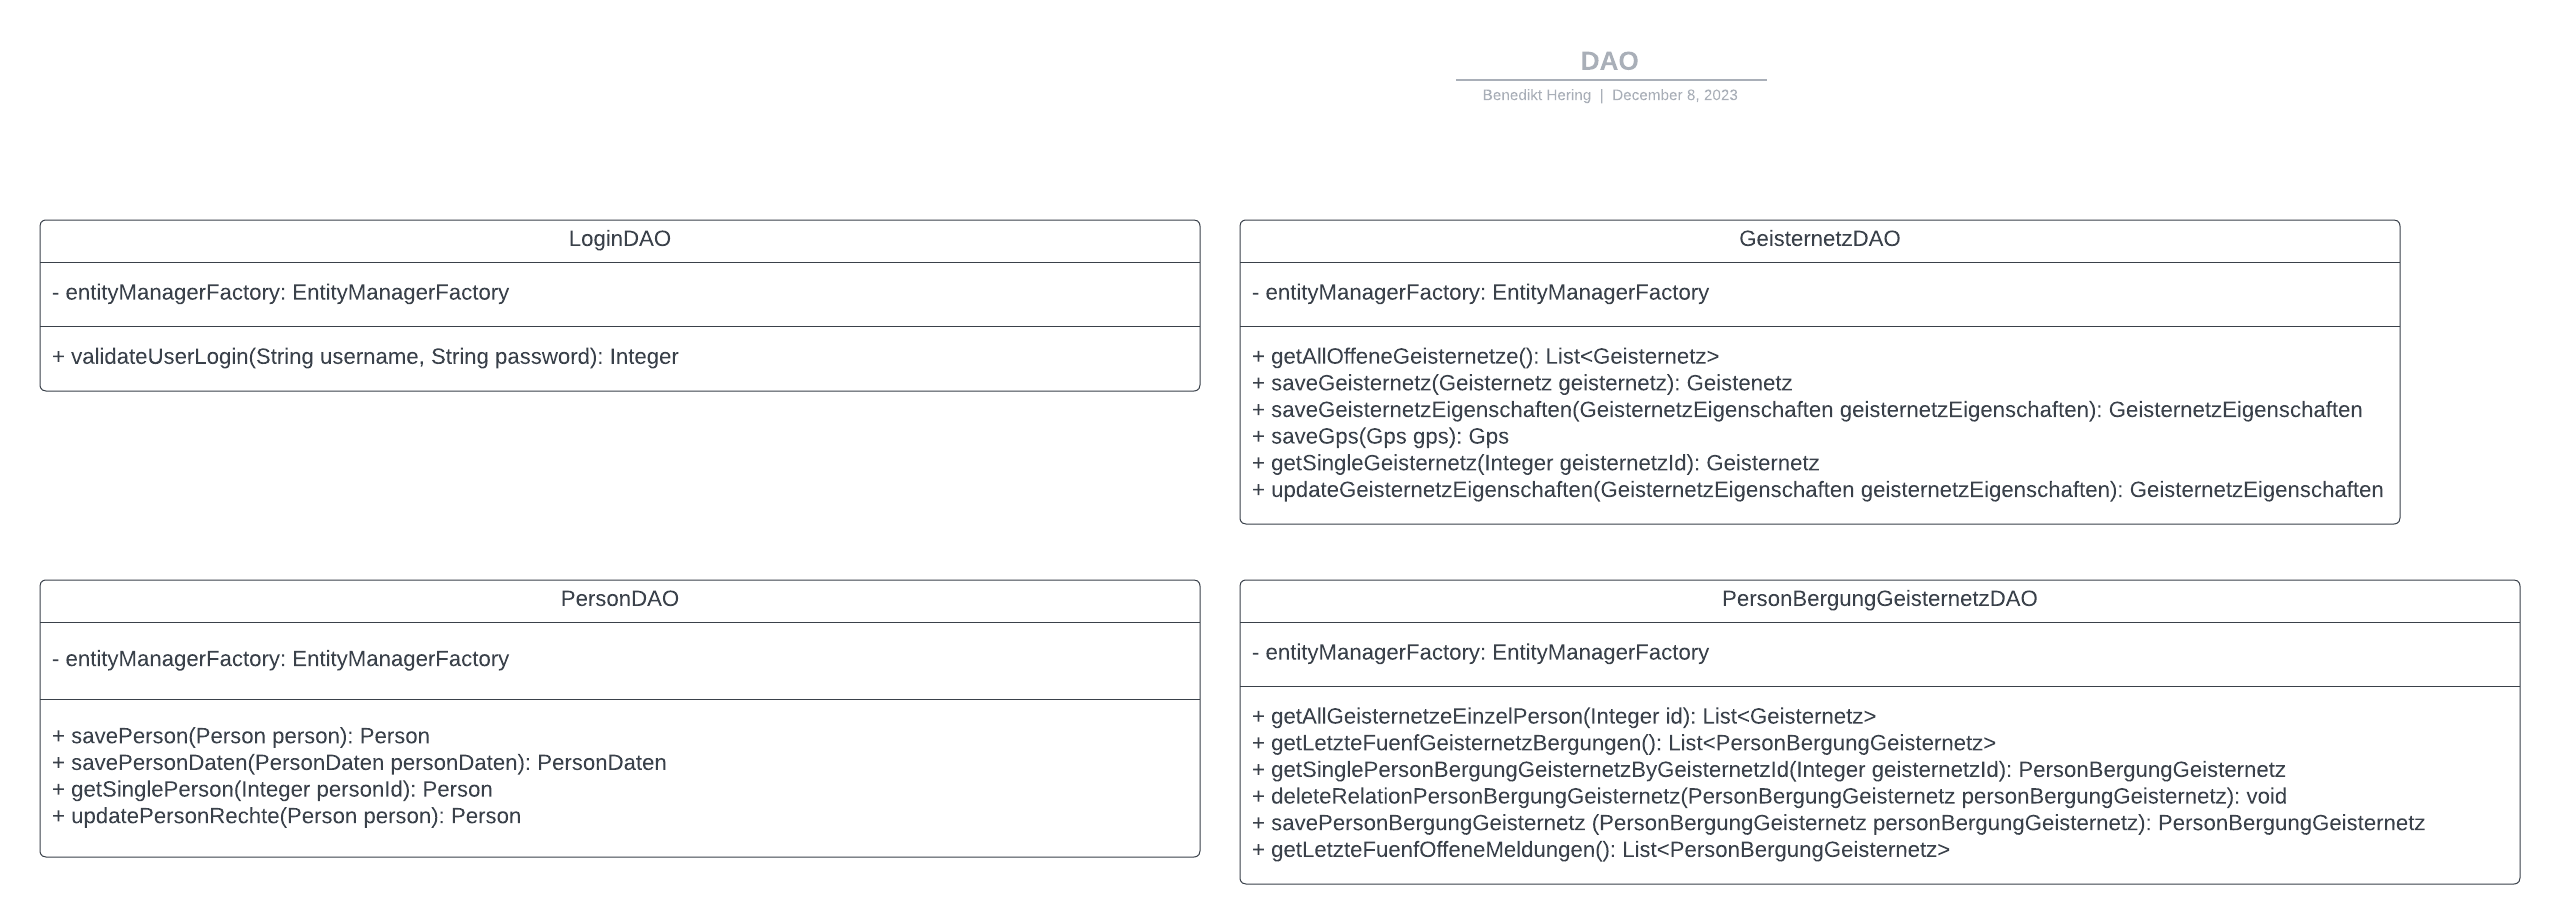
\includegraphics[width=\textwidth]{abbildungen/UML-DAO.png}
        \caption{Datenbankzugriffsobjekte UML}
        \label{uml-dao}
    \end{figure} 
    Um die Zugriffe auf die Datenbanktabellen zu steuern, werden Datenbankzugriffsobjekte verwendet.
    Diese Objekte steuern das Aktualisieren, Speichern oder Löschen von Entitäten.
    Eine beispielhafte Darstellung ist die Klasse PersonDAO. Sie enthält eine Methode, welche eine neue Person in der Datenbank speichert und eine Methode zum Aktualisieren der bereits bestehenden Personendaten.
    \begin{figure}[H]
        \centering
        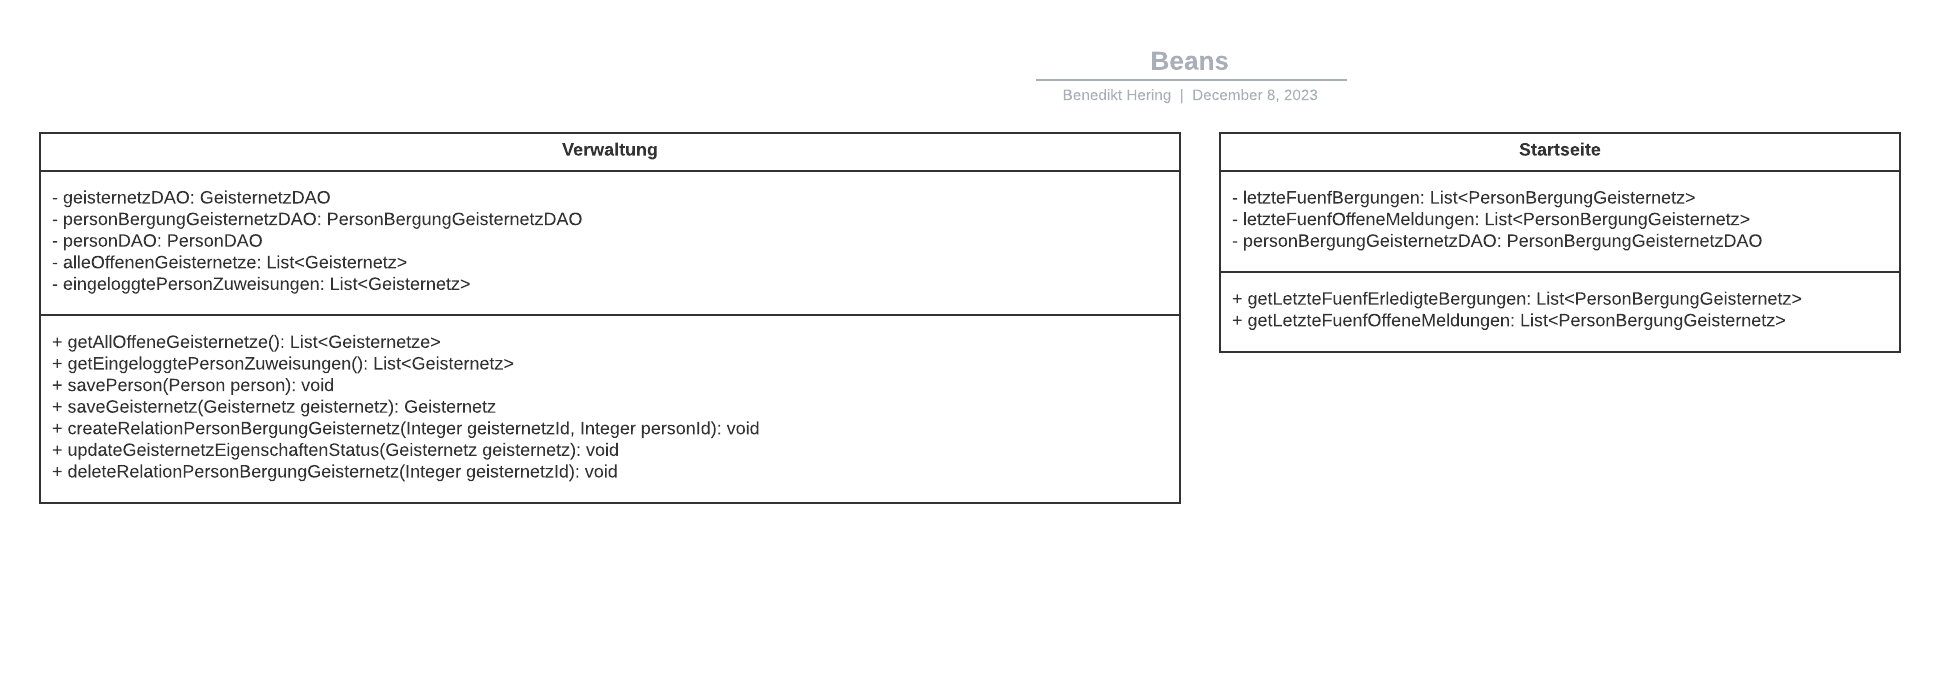
\includegraphics[width=\textwidth]{abbildungen/UML-Bean.png}
        \caption{Bean UML}
        \label{uml-bean}
    \end{figure} 
    Für die Verwaltung der Nutzerdaten sind die sogenannten Beans zuständig. In diesem Fall besteht die Webapplikation aus zwei Seiten, woraus zwei Beans die  Verwaltung.java 
    und Startseite.java resultieren. Da die Beans für die Verwaltung der Nutzerdaten zuständig sind, steuern diese unter anderem den Zugriff auf die Datenbankzugriffsobjekte. 
    Um die aktuelle Datenstruktur Endnutzer bereitzustellen, werden Listen für die Datenhaltung verwendet. So beinhaltet beispielsweise die Klasse Startseite.java die Liste namens „letzteFuenfOffeneBergungen“. Diese Liste beinhaltet stets die letzten fünf abgeschlossenen Bergungen und hat zusätzlich den Vorteil, dass nicht bei jedem Neuladen der Website 
    die Daten aus der Datenbank geladen werden müssen.
    \begin{figure}[H]
        \centering
        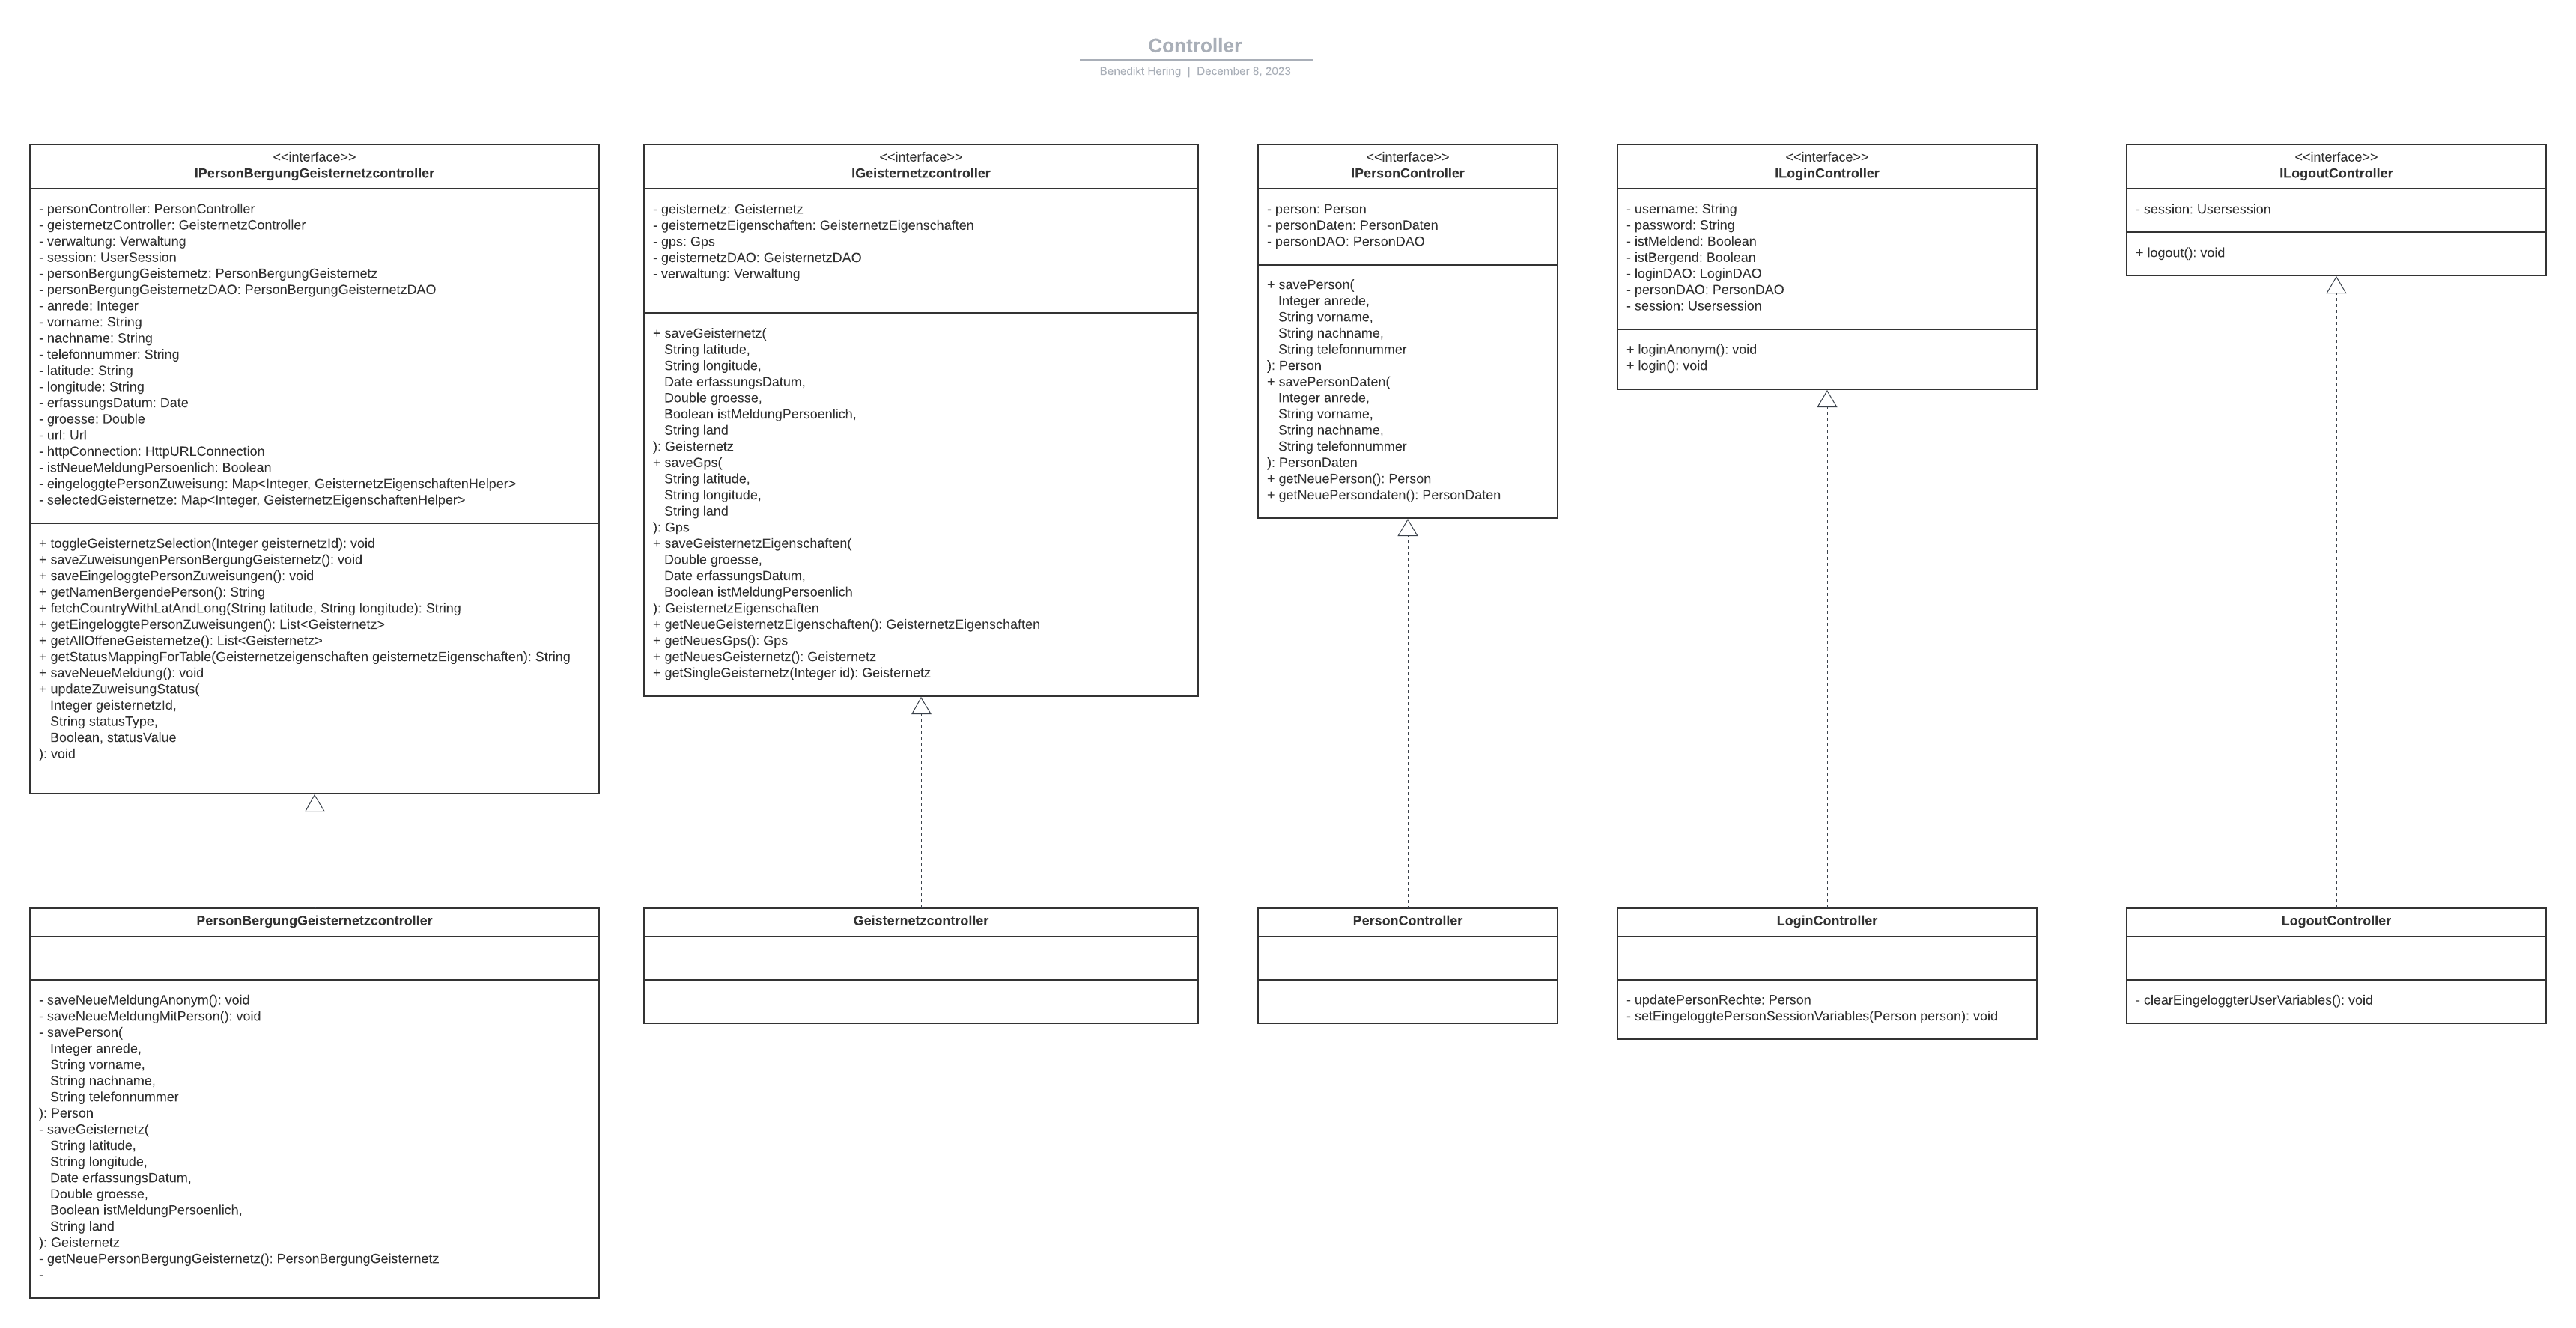
\includegraphics[width=\textwidth]{abbildungen/UML-Controller.png}
        \caption{Bean UML}
        \label{uml-controller}
    \end{figure} 
    Die nächste Abstraktionsebene stellen Controller dar. Diese steuern unter anderem die Beans und sind für das Entgegennehmen von Nutzereingaben zuständig.
    Der Unterschied von Controllern zu Beans ist, dass Controller spezifische Methoden für die Applikation bereitstellen. Ein gutes Beispiel dafür ist die Methode „fetchCountryWithLatAndLong“, welche den Ländername anhand des Latitudes und Longitudes über eine Schnittstelle abruft. 
    Im Gegensatz dazu speichern und verwalten die Beans lediglich die Daten der jeweiligen Seite.

    \newpage
    \subsubsection{Einrichtung der Entwicklungsumgebung}
    Um die Entwicklungsumgebung für den Entwicklungsprozess vorzubereiten, müssen einige Vorkehrungen getroffen
    werden. Zur Programmierung der Webapplikation wird die Entwicklungsumgebung IntelliJ Ultimate verwendet, die aufgrund
    des Studenten-Status zur kostenfreien Verwendung verfügbar ist. 
    Das Verwalten der Datenobjekte wird durch die Jakarta-Persistence-Api in Verbindung mit Hibernate verwendet. Um die Gestaltung der Benutzeroberflächen
    zu vereinfachen, wird die Css-Bibliothek Primefaces verwendet. Zur Verwendung der drei Pakete werden diese in der Datei „pom.xml“ eingebunden.
    \begin{figure}[H]
        \centering
        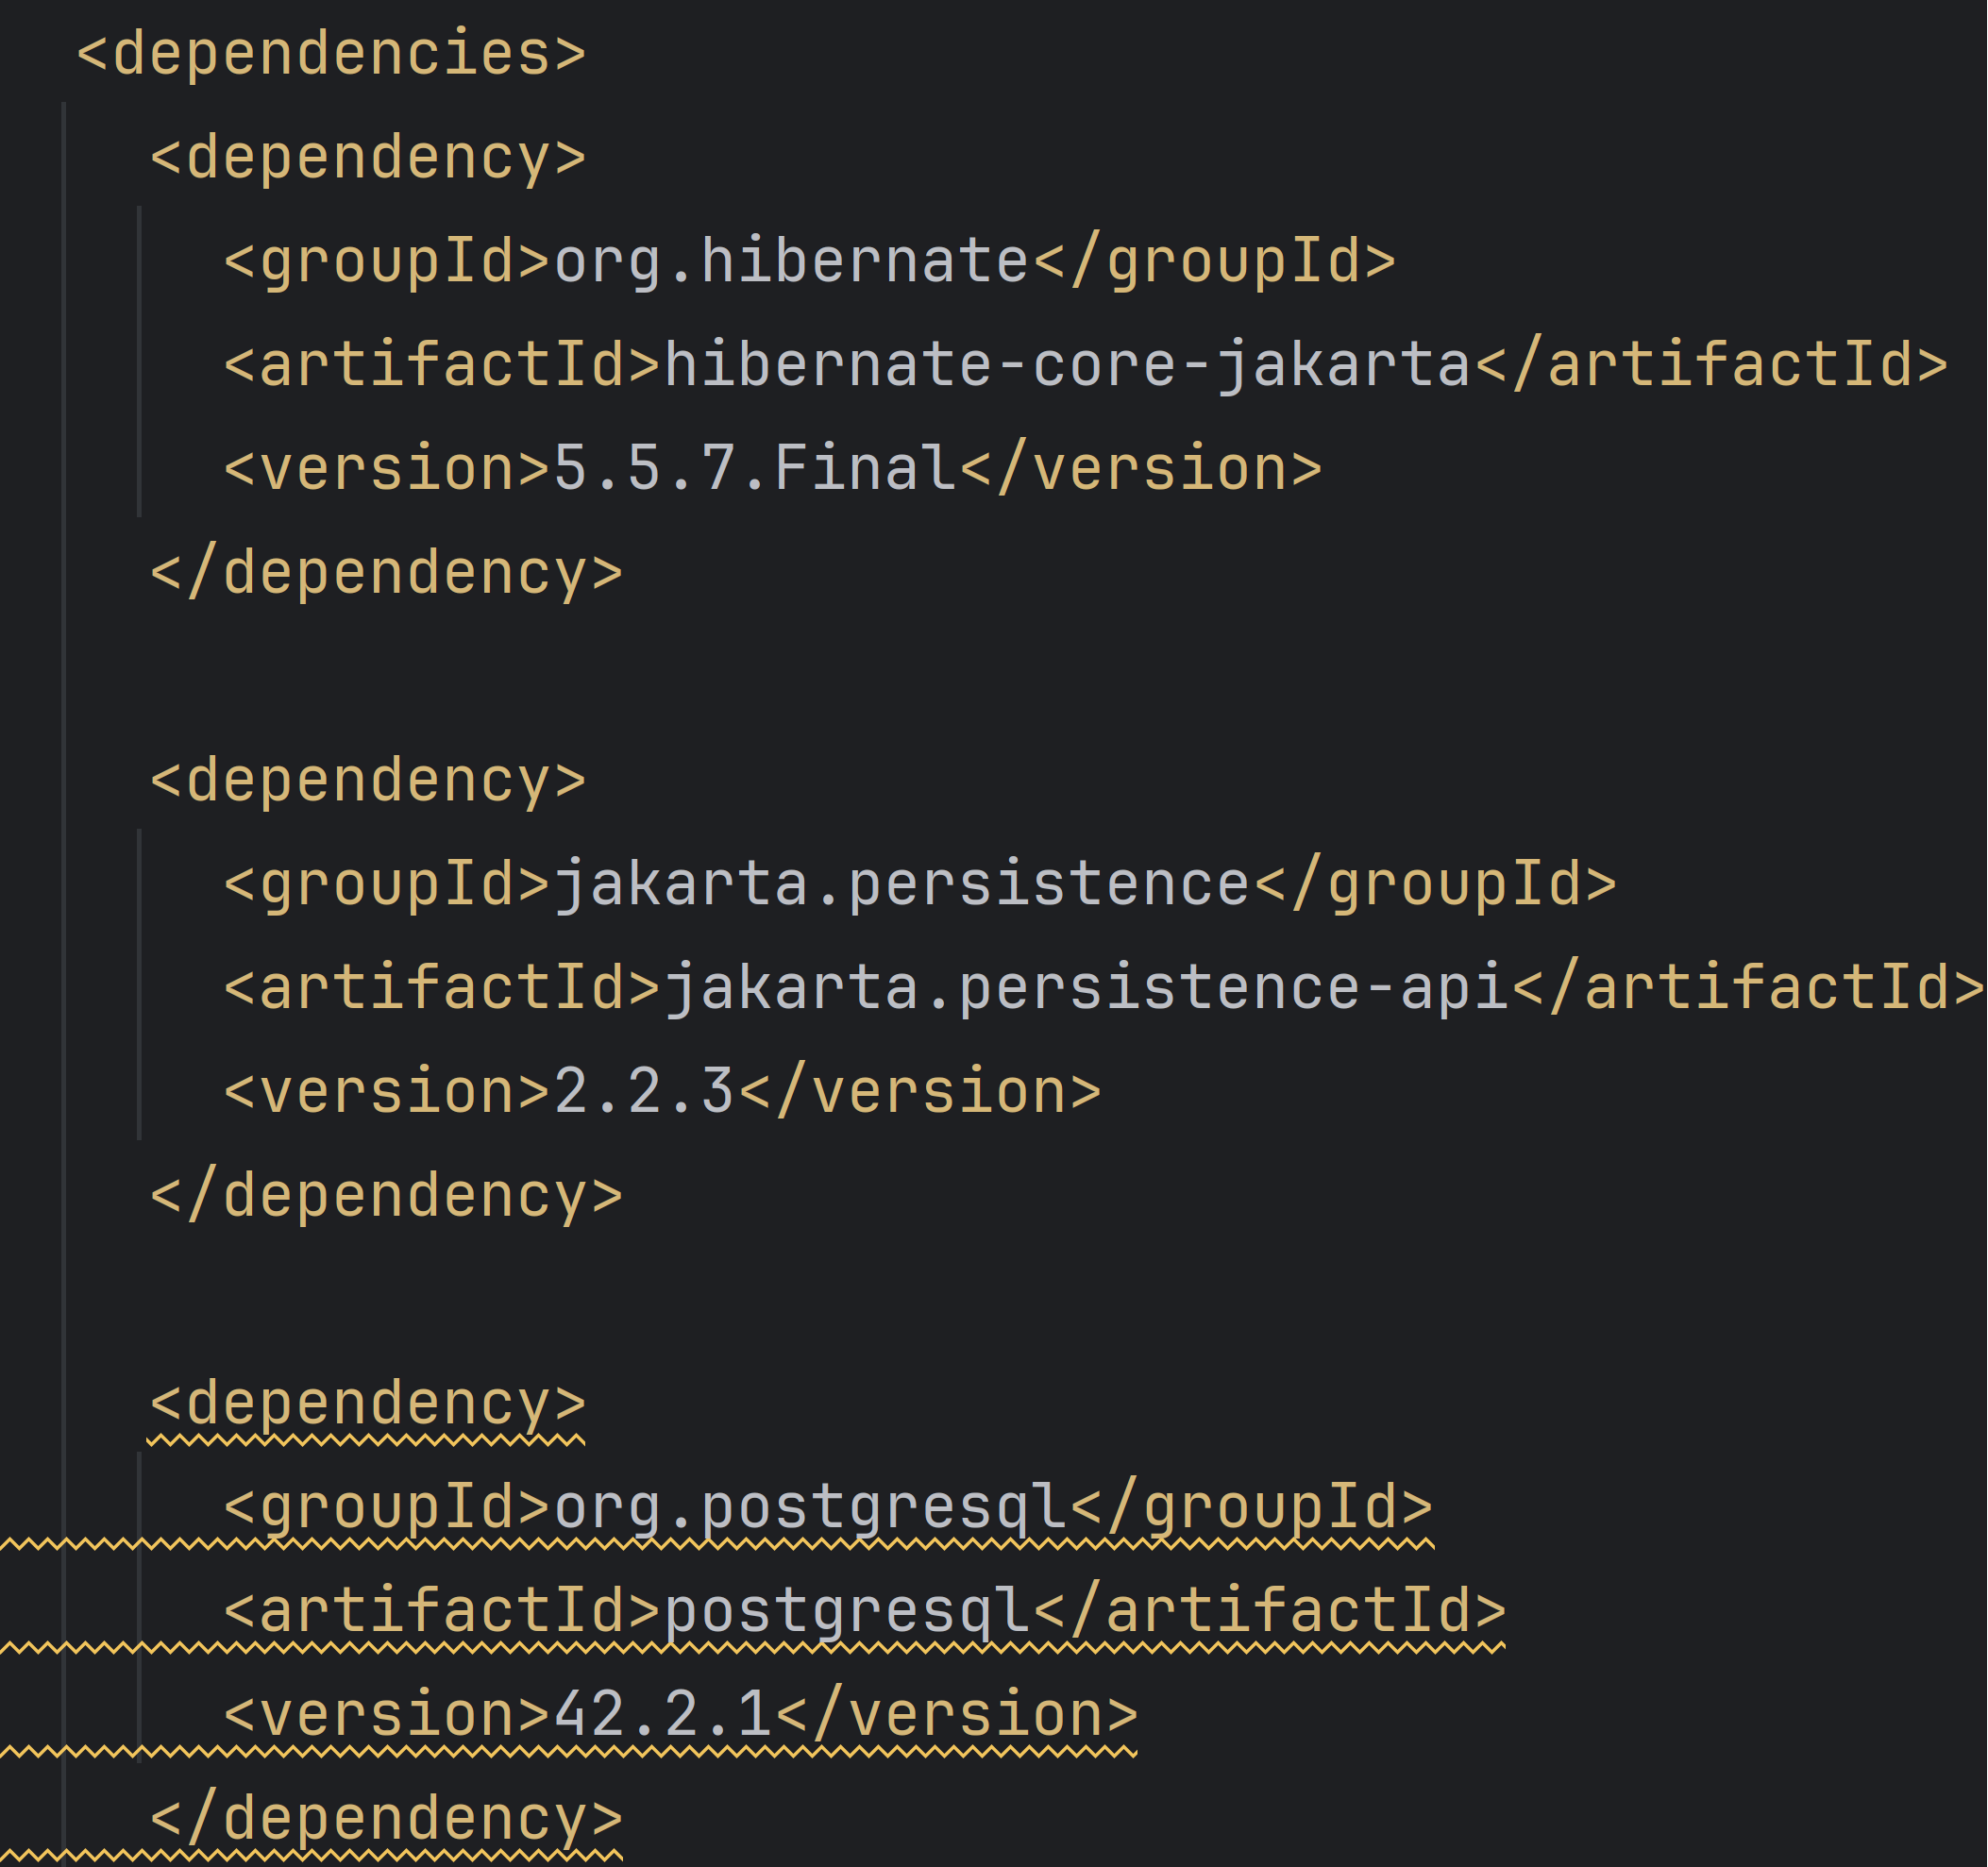
\includegraphics[width=\textwidth]{abbildungen/Pom-Xml.png}
        \caption{Pom.xml}
        \label{pom-xml}
    \end{figure}

    \newpage
    \subsubsection{Erstellung und Konfiguration der Datenbank}
    Begonnen wird mit der Erstellung der Datenbanktabellen. Innerhalb des Projekts wird die Datenbanktechnologie PostgreSQL verwendet, 
    welche für den Entwicklungsprozess auf dem lokalen Rechner zu installieren ist. Um die Verwaltung der Datenbankinstanz zu vereinfachen,
    wird das Datenbank-Management-System „pgAdmin“ verwendet. Letzteres stellt eine grafische Oberfläche zur Steuerung der PostgreSQL-Instanz bereit.
    Da die benötigte Datenstruktur im vorherigen Arbeitsschritt, in Form eines Entity-Relationship-Diagramms, bereits erstellt wurde, sind die Tabellen lediglich zu erstellen.
    Anschließend ist die lokale Datenbankinstanz mit dem Projekt zu verknüpfen. Dafür ist die Datei „persistence.xml“ mit den enstprechenden Konfigurationsdaten 
    der Datenbankinstanz und Tabellen innerhalb eines „persistence-unit“-Tags zu definieren.
    
    \newpage
    \subsubsection{Programmierung der Entitäten}
    Damit der Entity-Manager von Jakarta-Persistence mit Hibernate funktionsfähig ist, müssen die dort hinterlegten Klassen als Entitäten im Quellcode erstellt werden. Jede Entität 
    stellt eine Datenbanktabelle in Form einer Klasse im Quellcode dar.
    Die einzelnen Klassen dürfen lediglich eine leeren Konstruktur und Getter- und Setter-Methoden für die Attribute beinhalten.
    Damit die Java-Klasse als Entität erkannt wird, benötigt diese die Annotationen Entity und Tablename, letzterer definiert den Tabellenname. 
    Anschließend muss jede Spalte, welche innerhalb der Tabelle vorhanden ist, als Attribut der Klasse kodiert werden.
    \begin{figure}[H]
        \centering
        \includegraphics[width=\textwidth]{abbildungen/Geisternetz-Entiät.png}
        \caption{Geisternetz Entität}
        \label{geisternetz-entitaet}
    \end{figure} 
    In Betrachtung des Beispiels der Klassenentität Geisternetz sind ebenfalls einige Besonderheiten zu beachten. Als erster Attribut
    wird der Primärschlüssel der Tabelle definiert. Dieser benötigt die Annotationen Id und GeneratedValue, welche
    die automatische Generierung eines aufsteigenden Schlüsselwertes definiert. Um die gewollte Spalte zu referenzieren, wird
    durch die Annotation Column der entsprechende Spaltenname als Wert hinterlegt.
    Die beiden weiteren Attribute, GeisternetzEigenschaften und Gps, stellen eine Fremdschlüsselbeziehung zu der jeweiligen verknüpften Relationstabelle dar.
    Da in diesem Fall eine Eins-Zu-Eins-Beziehung vorliegt, wird die Annotation OneToOne gewählt. Um die jeweilige Spalte innerhalb der Tabelle zu
    adressieren, wird die ergänzende Annotation JoinColumn verwendet. Letztere Annotation hinterlegt die Spalte innerhalb der Tabelle Geisternetz und die zu referenzierende Spalte
    innerhalb der Tabelle GeisternetzEigenschaften.
    Um die Steuerung der Werte zu gewährleisten, werden die Getter- und Setter-Methoden erstellt. Zu beachten ist, dass die Spalte Id
    lediglich eine Getter-Methoden besitzen darf, da dessen Wert automatisch generiert wird. Bei einer manuellen Manipulation der
    Identifikator-Generierung ist eine hohe Fehleranfälligkeit vorhanden, welche mögliche Inkonsistenzen birgt.
    \\
    Hingegen zum obigen Beispiel stellt die dort referenzierte Entität, GeisternetzEigenschaften, eine einfachere Struktur dar.
    Innerhalb dieser wird wie zuvor der Primärschlüssel durch die Verwendung der Annotationen Id, GeneratedValue und
    Column erstellt. Anschließend werden die jeweiligen Spalten mit der Annotation Column dort erstellt.
    Schlussendlich werden die entsprechenden Getter- und Setter-Methoden der jeweiligen Attribute zu erstellen.

    \newpage
    \subsubsection{Programmierung der Datenbankzugriffsobjekte}
    Die zuvor erstellten Entitätsklassen werden durch Datenbankzugriffsobjekte verwaltet. Ein Datenbankzugriffsobjekt steuert die Erstellung, Löschung und Manipulation von Entitäten.
    Durch das bereits erstellte Uml-Diagramm ist die Struktur der einzelnen Datenbankzugriffsobjekte ebenfalls vorgegeben.
    \begin{figure}[H]
        \centering
        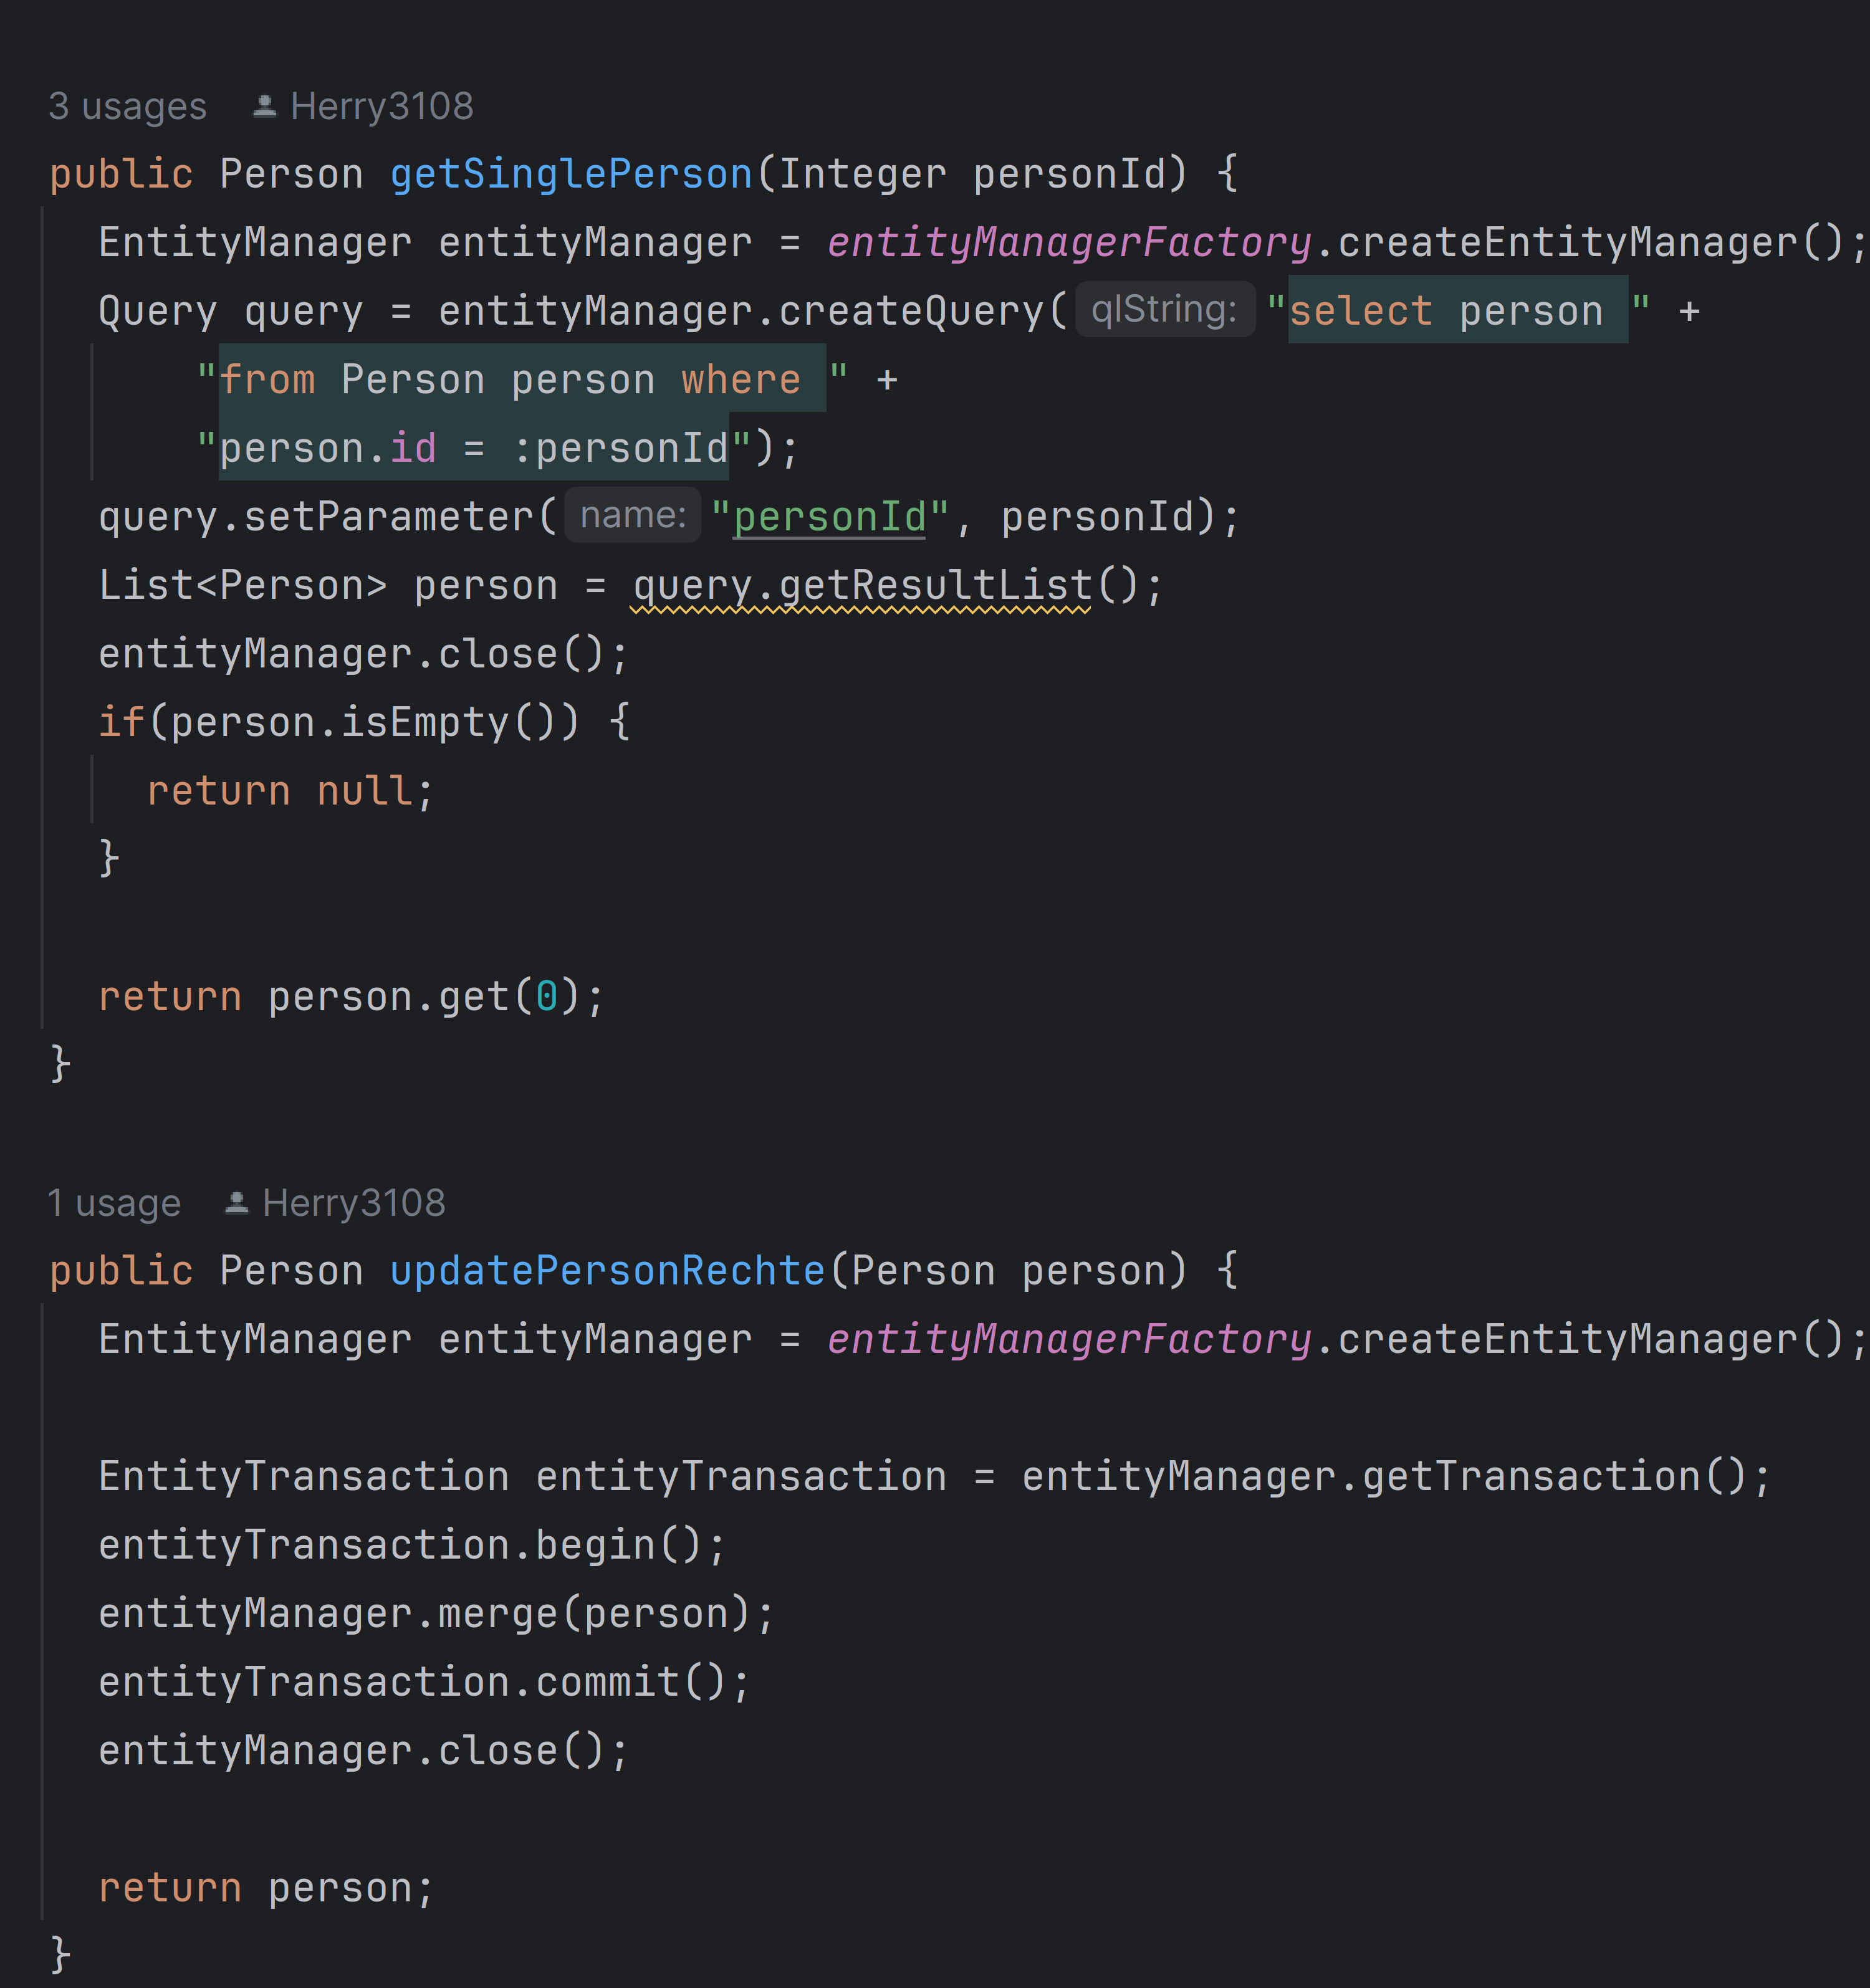
\includegraphics[width=\textwidth]{abbildungen/Person-DAO.png}
        \caption{PersonDAO}
        \label{person-dao}
    \end{figure} 

    \newpage
    Eine beispielhafte Programmierung stellt die Datei PersonDAO.java dar. 
    Innerhalb der Klasse wird eine private Konstante vom Typ EntityManagerFactory initialisiert. Durch die Verwendung
    der createEntityManager-Methode dieser Klasse wird eine Instanz des Entity-Managers in der jeweiligen Methode erzeugt.
    Bei der Programmierung der Methode namens „getSinglePerson(Integer personId)“ ist die Verwendung des Entity-Managers demonstriert.
    Zu Beginn der Methode wird die Instanz des Entity-Managers erstellt. Anschließend wird durch die Verwendung des Befehls 
    „entityManager.createQuery("select person from Person person where person.id = :personId")“ eine Datenkabfrageobjekt vom 
    Klassentyp Query mit dem hinterlegten Suchtbegriff erstellt. Innerhalb des Suchbegriffs wird per ":personId" ein Parameter adressiert, welcher zu definieren gilt.
    Der gewünschte Parameter wird über die Methode „setParameter("personId", personId)“ erstellt. Durch diese Schritte ist das Objekt für die Datenbankabfrage definiert.
    Im nächsten Schritt gilt es die Suchabfrage durch die Methode „getResultList()“ zu starten, welche die Suchergebnisse als Liste zurückgibt.
    Da die Suchabfrage vollendet ist, gilt es die Instanz Entity-Managers durch die Methode „entityManager.close()“ zu schließen und das Ergebnis zu verarbeiten.
    Sollte das Suchergebnis einen leeren Inhalt ausweisen, ist keine Person zum gesuchten Identifikator auffindbar und der Rückgabewert beträgt „null“.
    Ist hingegen ein Suchergebnis vorhanden, wird die entsprechende Person zurückgegen. In diesem Fall ist das Suchergebniss aufgrund des gesuchten Primärschlüssels auf maximal einen Inhalt limitiert.

    \newpage
    \subsubsection{Programmierung der Beans am Beispiel Verwaltung}
    In diesem Schritt werden die Beans programmiert, welche für die Verwaltung der Benutzerdaten zuständig sind.
    \begin{figure}[H]
        \centering
        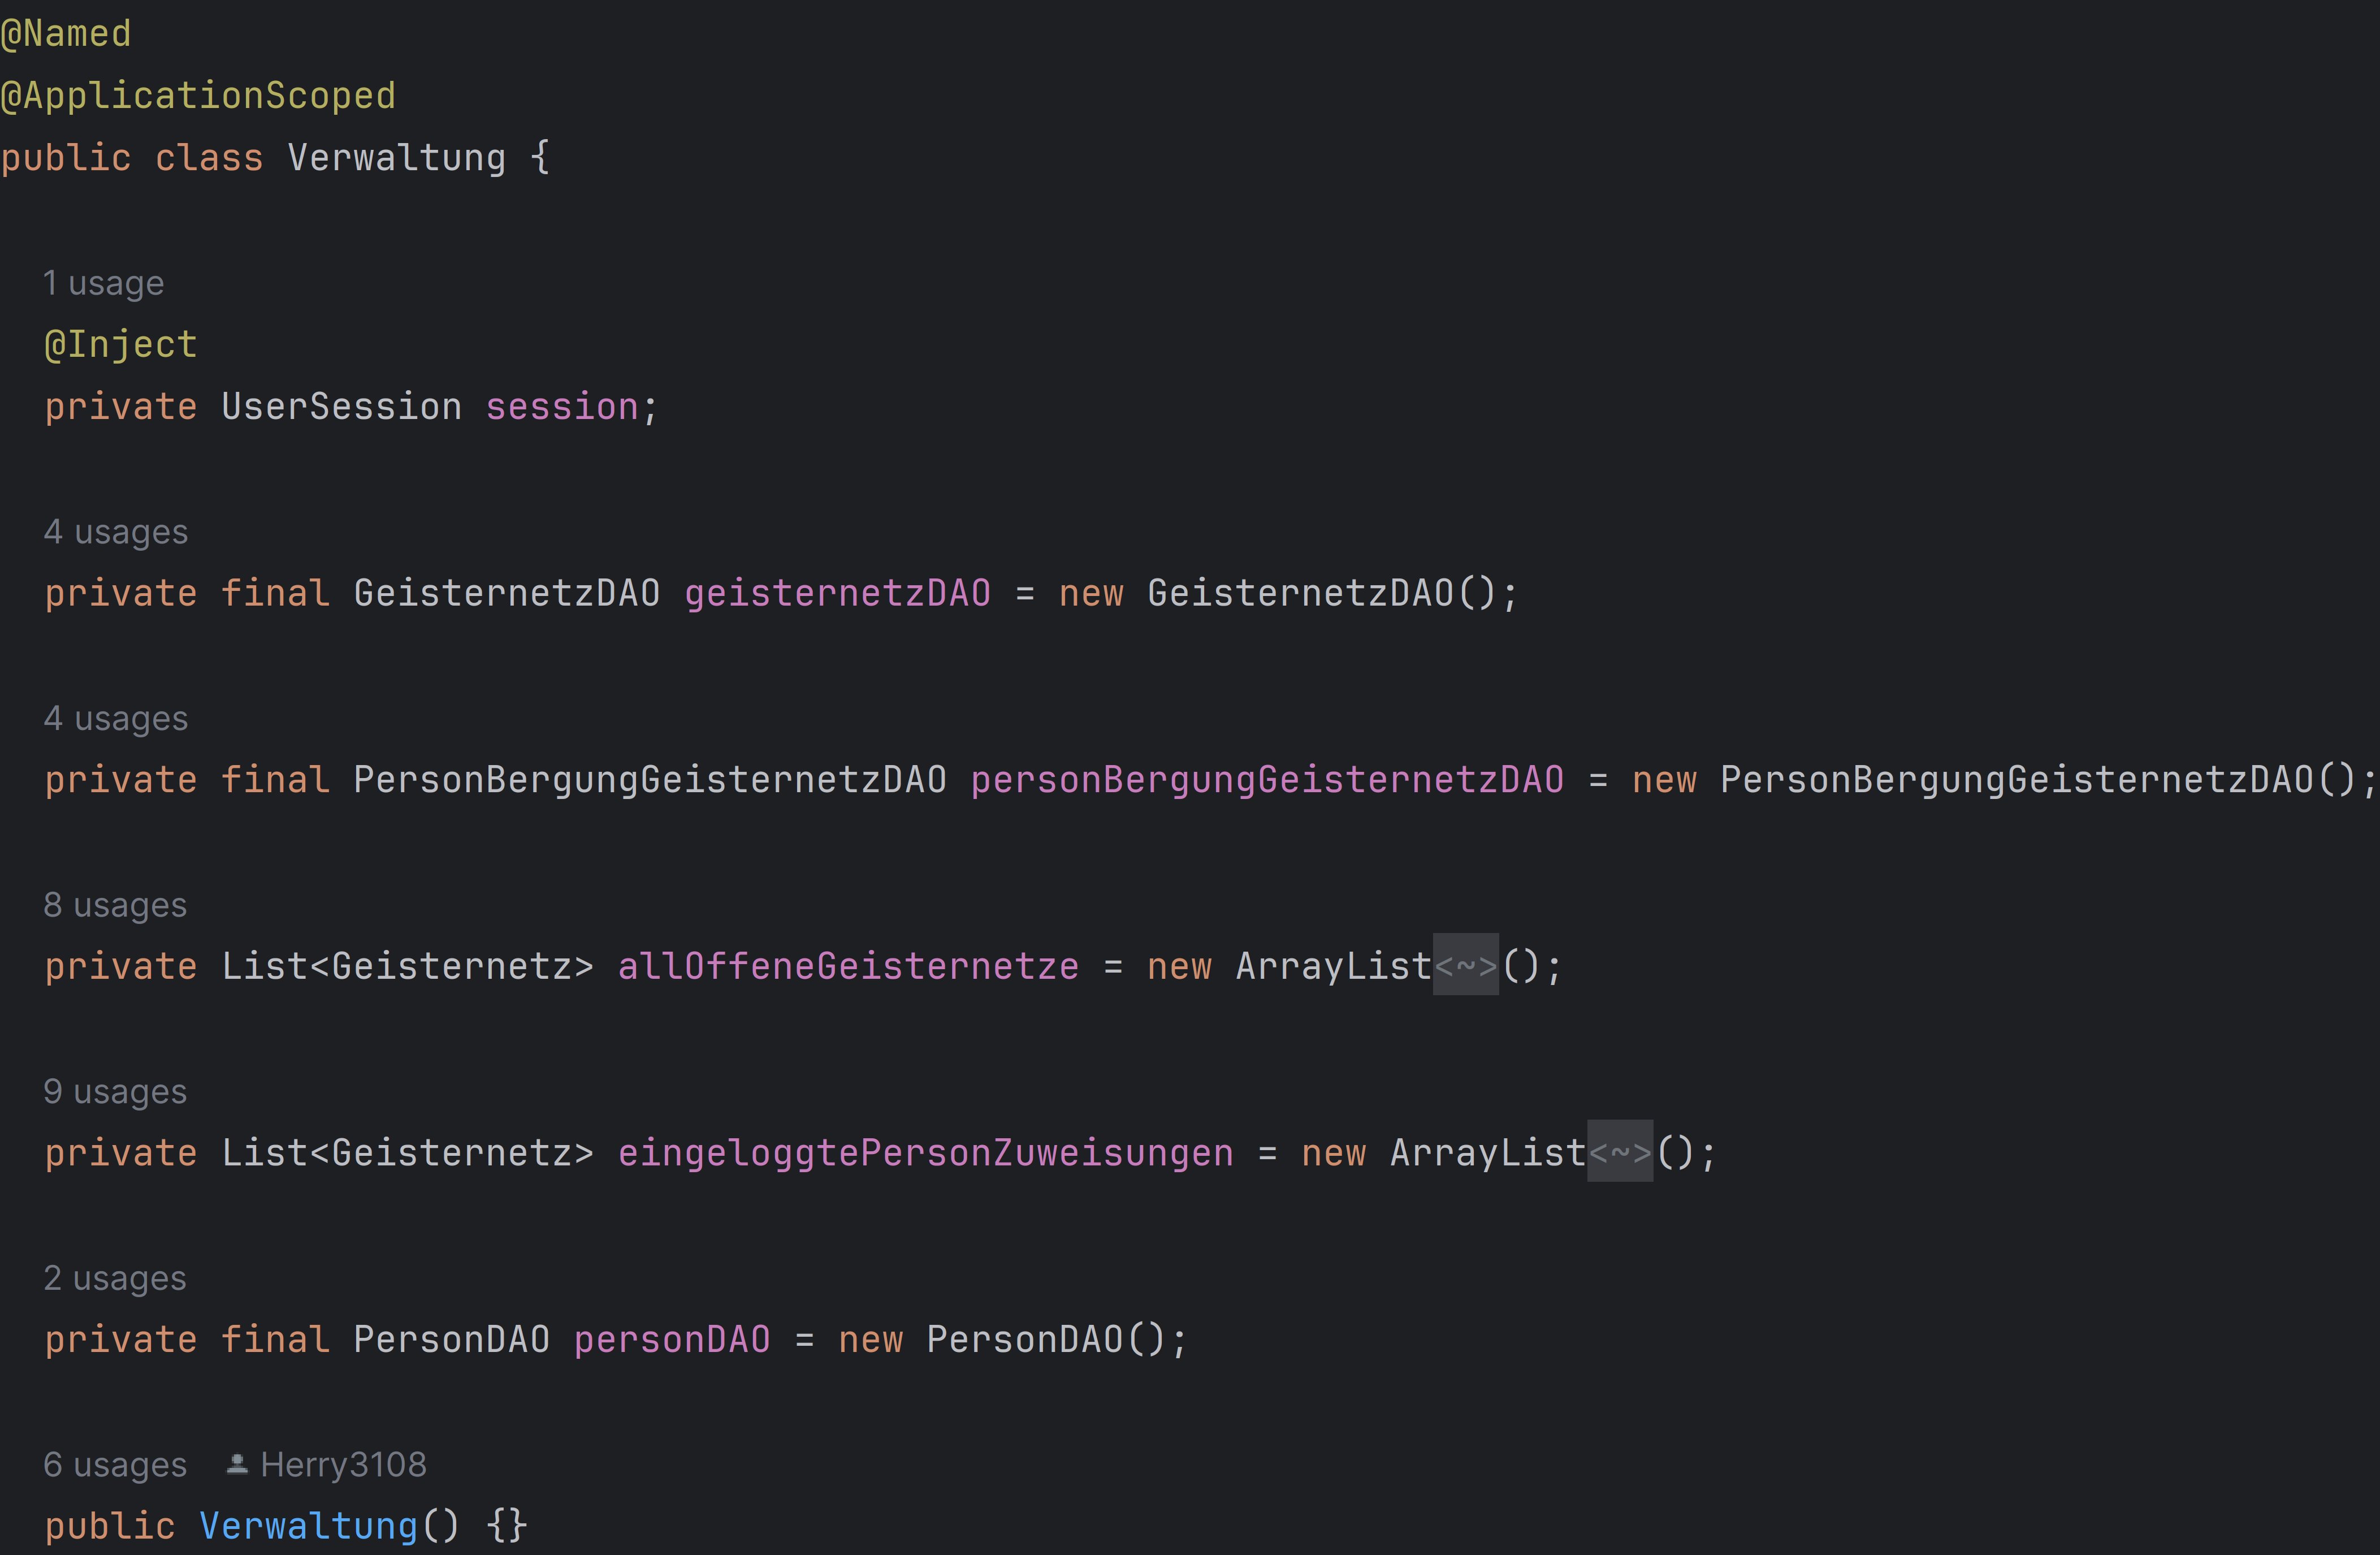
\includegraphics[width=\textwidth]{abbildungen/Verwaltung-Bean-Teil-1.png}
        \caption{Verwaltung Bean Teil 1}
        \label{verwaltung-bean-teil-1}
    \end{figure} 
    Um die Bean für die Verwaltungsseite zu erstellen, wird zuerst eine Klasse namens Verwaltung.java erstellt und mit den Annotationen Named und ApplicationScoped versehen. 
    Anschließend werden die Attribute der Klasse definiert. Um das Prinzip der Datenkapselung einzuhalten, welches die Steuerung der Attribut-Werte von außen
    lediglich über Methoden zulässt, werden die Attribute stets mit einem privaten Gültigkeitsbereich versehen.
    \begin{figure}[H]
        \centering
        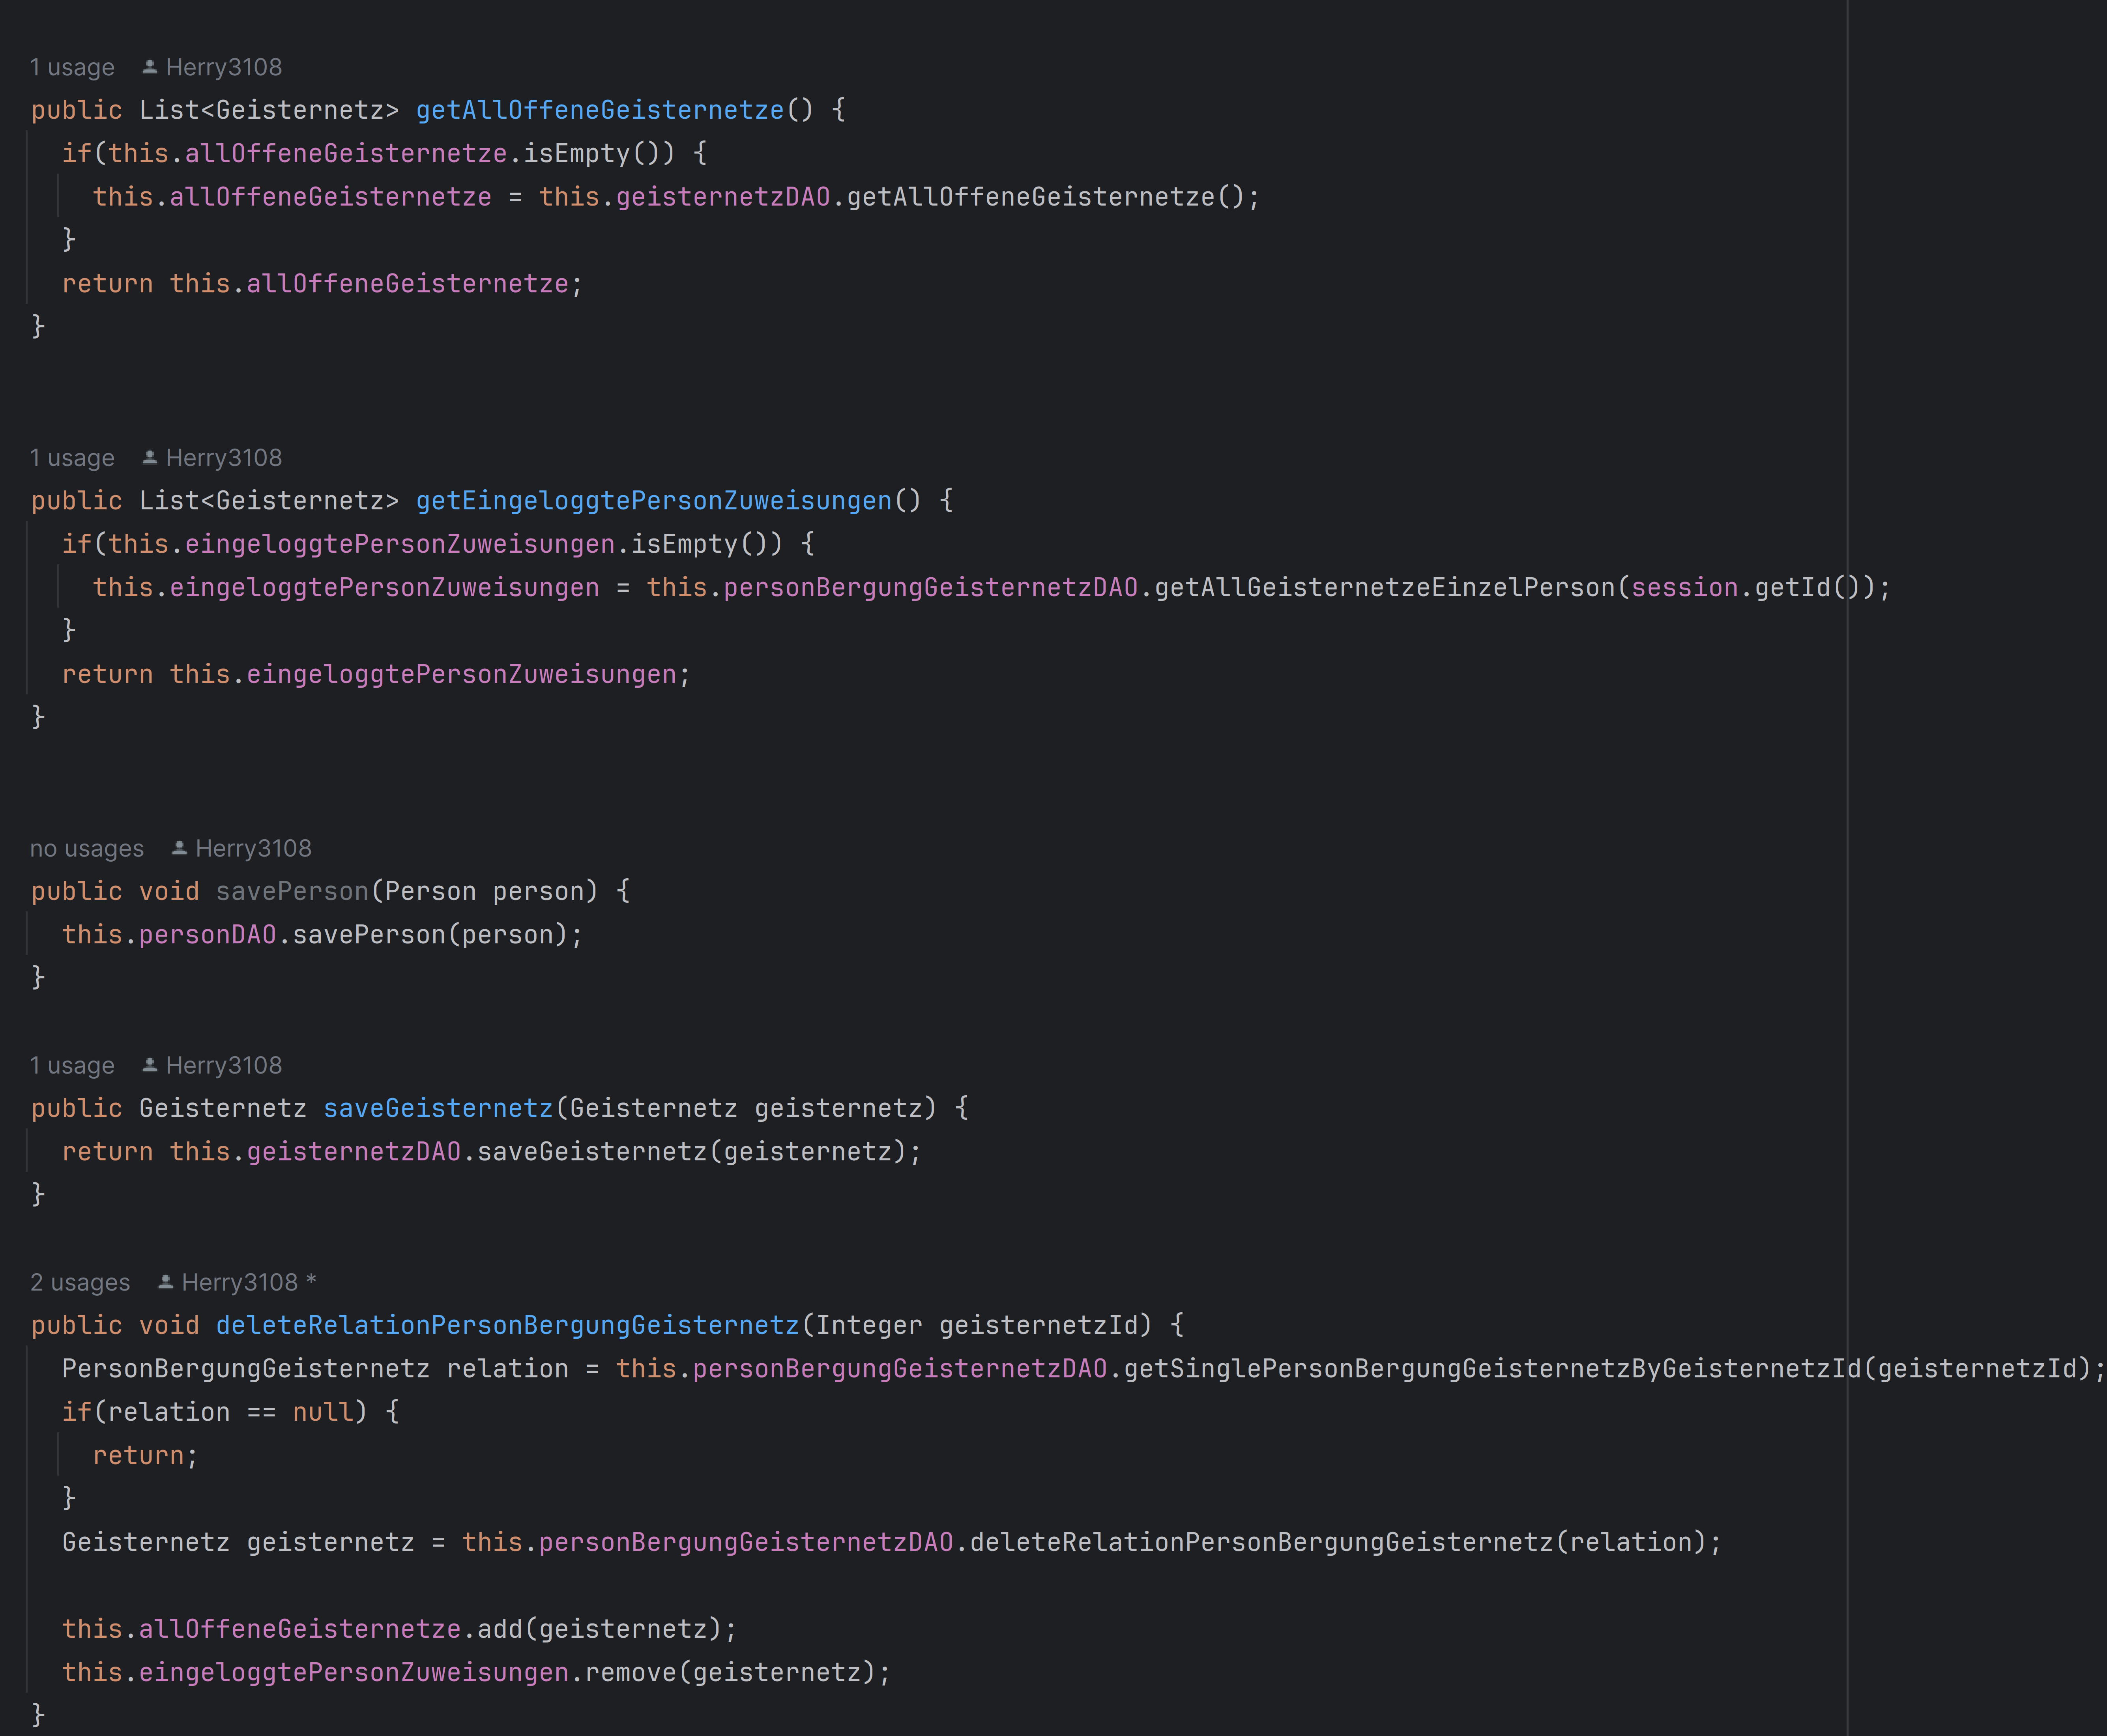
\includegraphics[width=\textwidth]{abbildungen/Verwaltung-Bean-Teil-2.png}
        \caption{Verwaltung Bean Teil 2}
        \label{verwaltung-bean-teil-2}
    \end{figure} 
    Um zusätzlich die Verwaltung der Daten zu ermöglichen, werden Methoden definiert. Soll beispielsweise ein neues
    Geisternetz gespeichert werden, muss dafür eine Methode verfügbar sein. Durch die Erstellung der Methode saveGeisternetz(Geisternetz geisternetz) wird die Speicherung eines neuen Geisternetzes ermöglicht.
    Innerhalb dieser Methode wird das neue Objekt durch Verwendung des Datenbankzugriffsobjekt namens „geisternetzDAO“ zuerst in der Datenbank gespeichert. Anschließend wird das Objekt in die Liste „offeneGeisternetze“ hinzugefügt, um die 
    Datenhaltung der Seite aktuell zu halten.
    
    \newpage
    \subsubsection{Programmierung der Controller am Beispiel PersonBergungGeisternetzController}
    Die Struktur der benötigten Klasse, PersonBergungGeisternetzController, und des Interfaces, IPersonBergungGeisternetzController, wurde durch das korrespondierende UML-Diagramm definiert.
    \begin{figure}[H]
        \centering
        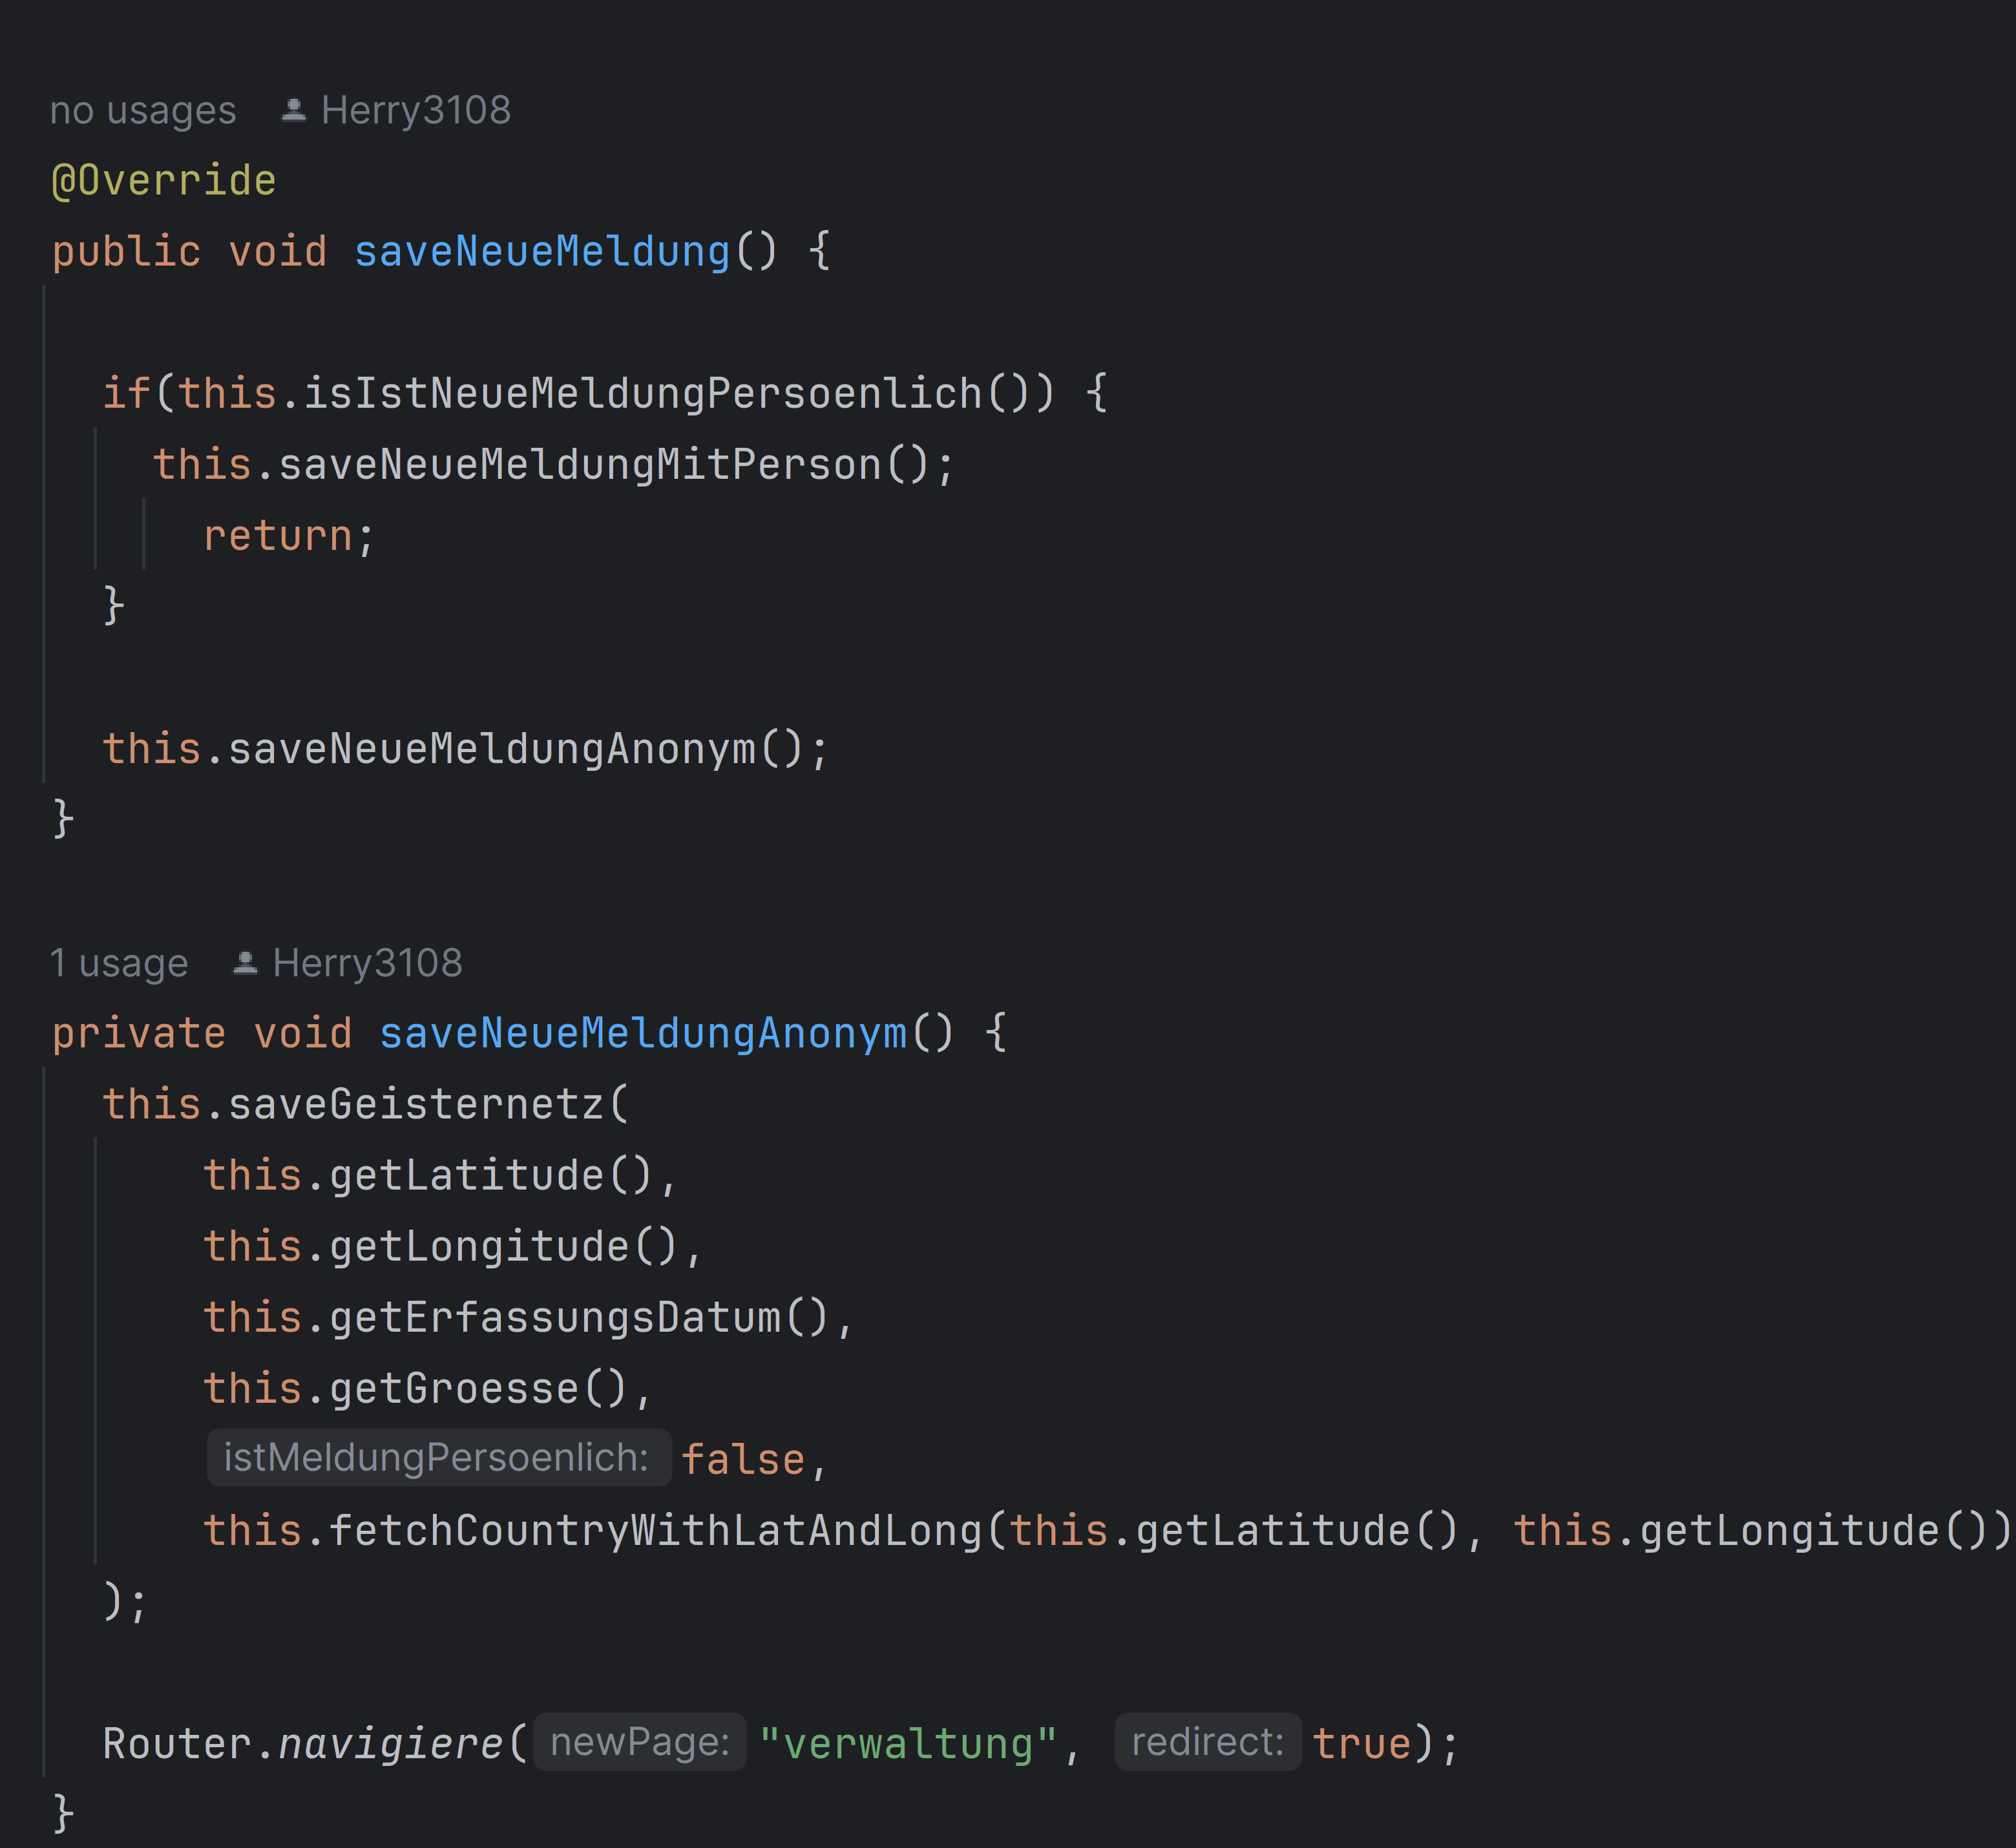
\includegraphics[width=\textwidth]{abbildungen/PersonBergungGeisternetzController.png}
        \caption{PersonBergungGeisternetzController}
        \label{person-bergung-geisternetz-controller}
    \end{figure} 

    \newpage
    Innerhalb der Controller-Klasse sind zu Beginn vier weitere Jakarta-Objekte zu referenzieren. Da diese einen eigenen Gültigkeitsbereich innerhalb von Jakarta EE besitzen, sind sie nicht zu instanziieren, sondern per Injektion zu steuern.
    Um die Injektion zu gewährleisten, wird das Attribut wie gewohnt mit einem privaten Gültigkeitsbereich innerhalb der Klasse versehen und erhält zusätzlich
    die Annotation namens „Inject“. Dies hat die Besonderheit, dass die Attribute auch ohne Getter- und Setter-Methoden innerhalb der Klasse verwendbar sind.
    Die weiteren Klasse-Attribute werden lediglich mit dem Gültigkeitsbereich „privat“ versehen und per Getter- und Setter-Methoden verwaltet.
    Die Funktion der Controller innerhalb der Anwendung bezieht sich primär auf die Aufbereitung der Nutzerdaten in Objekte, wie auch die Schnittstellenabrufe von Daten.
    Eine Aufbereitung der Nutzerdaten stellt die Methode „saveNeueMeldungAnonym()“ dar. Der Controller besitzt alle nötigen Attribute zur Erstellung einer neuen anonymen Meldung, welche durch die Erstellung einer neuen Geisternetz-Entität umgesetzt wird.
    Innerhalb der Methode selbst wird der GeisternetzController referenziert. Dieser erstellt die beiden Entitäten GeisternetzEigenschaften und Gps durch die Verwendung des GeisternetzDAO's. Folgend wird das Geisternetz selbst in der Datenbank 
    persistiert und innerhalb der Bean Verwaltung in passende Listenattribut aufgenommen. Anschließend wird das Neuladen der Seite gestartet, um die Endnutzeransicht der Webapplikation zu aktualisieren.
    
    \newpage
    \subsubsection{Programmierung des Frontend am Beispiel der Verwaltungsseite}
    Die Entwicklung des Backend ist soweit abgeschlossen. Damit die Webapplikation funktionsfähig wird, muss das Frontend ebenfalls programmiert werden.
    Wie zu Beginn bereits erwähnt, wir dieses unter Verwendung des Framework Primefaces erstellt.
    Die Dateien im Frontend, müssen im Gegensatz zum Backend, keine Java-, sondern XHTML-Dateien sein. Aus diesem Grund wird eine Datei namens „verwaltung.xhtml“ erstellt.
    Als Erstes muss innerhalb der Datei der Xhtml- und Html-Tag mit den gewünschten Abhängigkeiten gesetzt werden. Um den Header mit inkludiertem Navigationsmenü erstellen,
    wird mit einem div-Tag und dessen Attribut „id='header'“ gestartet. Damit das zu erstellende Navigationsmenü auf andere Seiten verweisen kann, ist ein ummantelndes h:form-Tag nötig. Innerhalb des ummantelnden Tags wird die Struktur des Menüs durch die Verwendung der 
    p:menubar- und p:menuitem-Tags definiert. Die Funktionalität zum Wechseln der Seiten wird über eine Methode in der Klasse Router gesteuert.
    
    \newpage
    \begin{figure}[H]
        \centering
        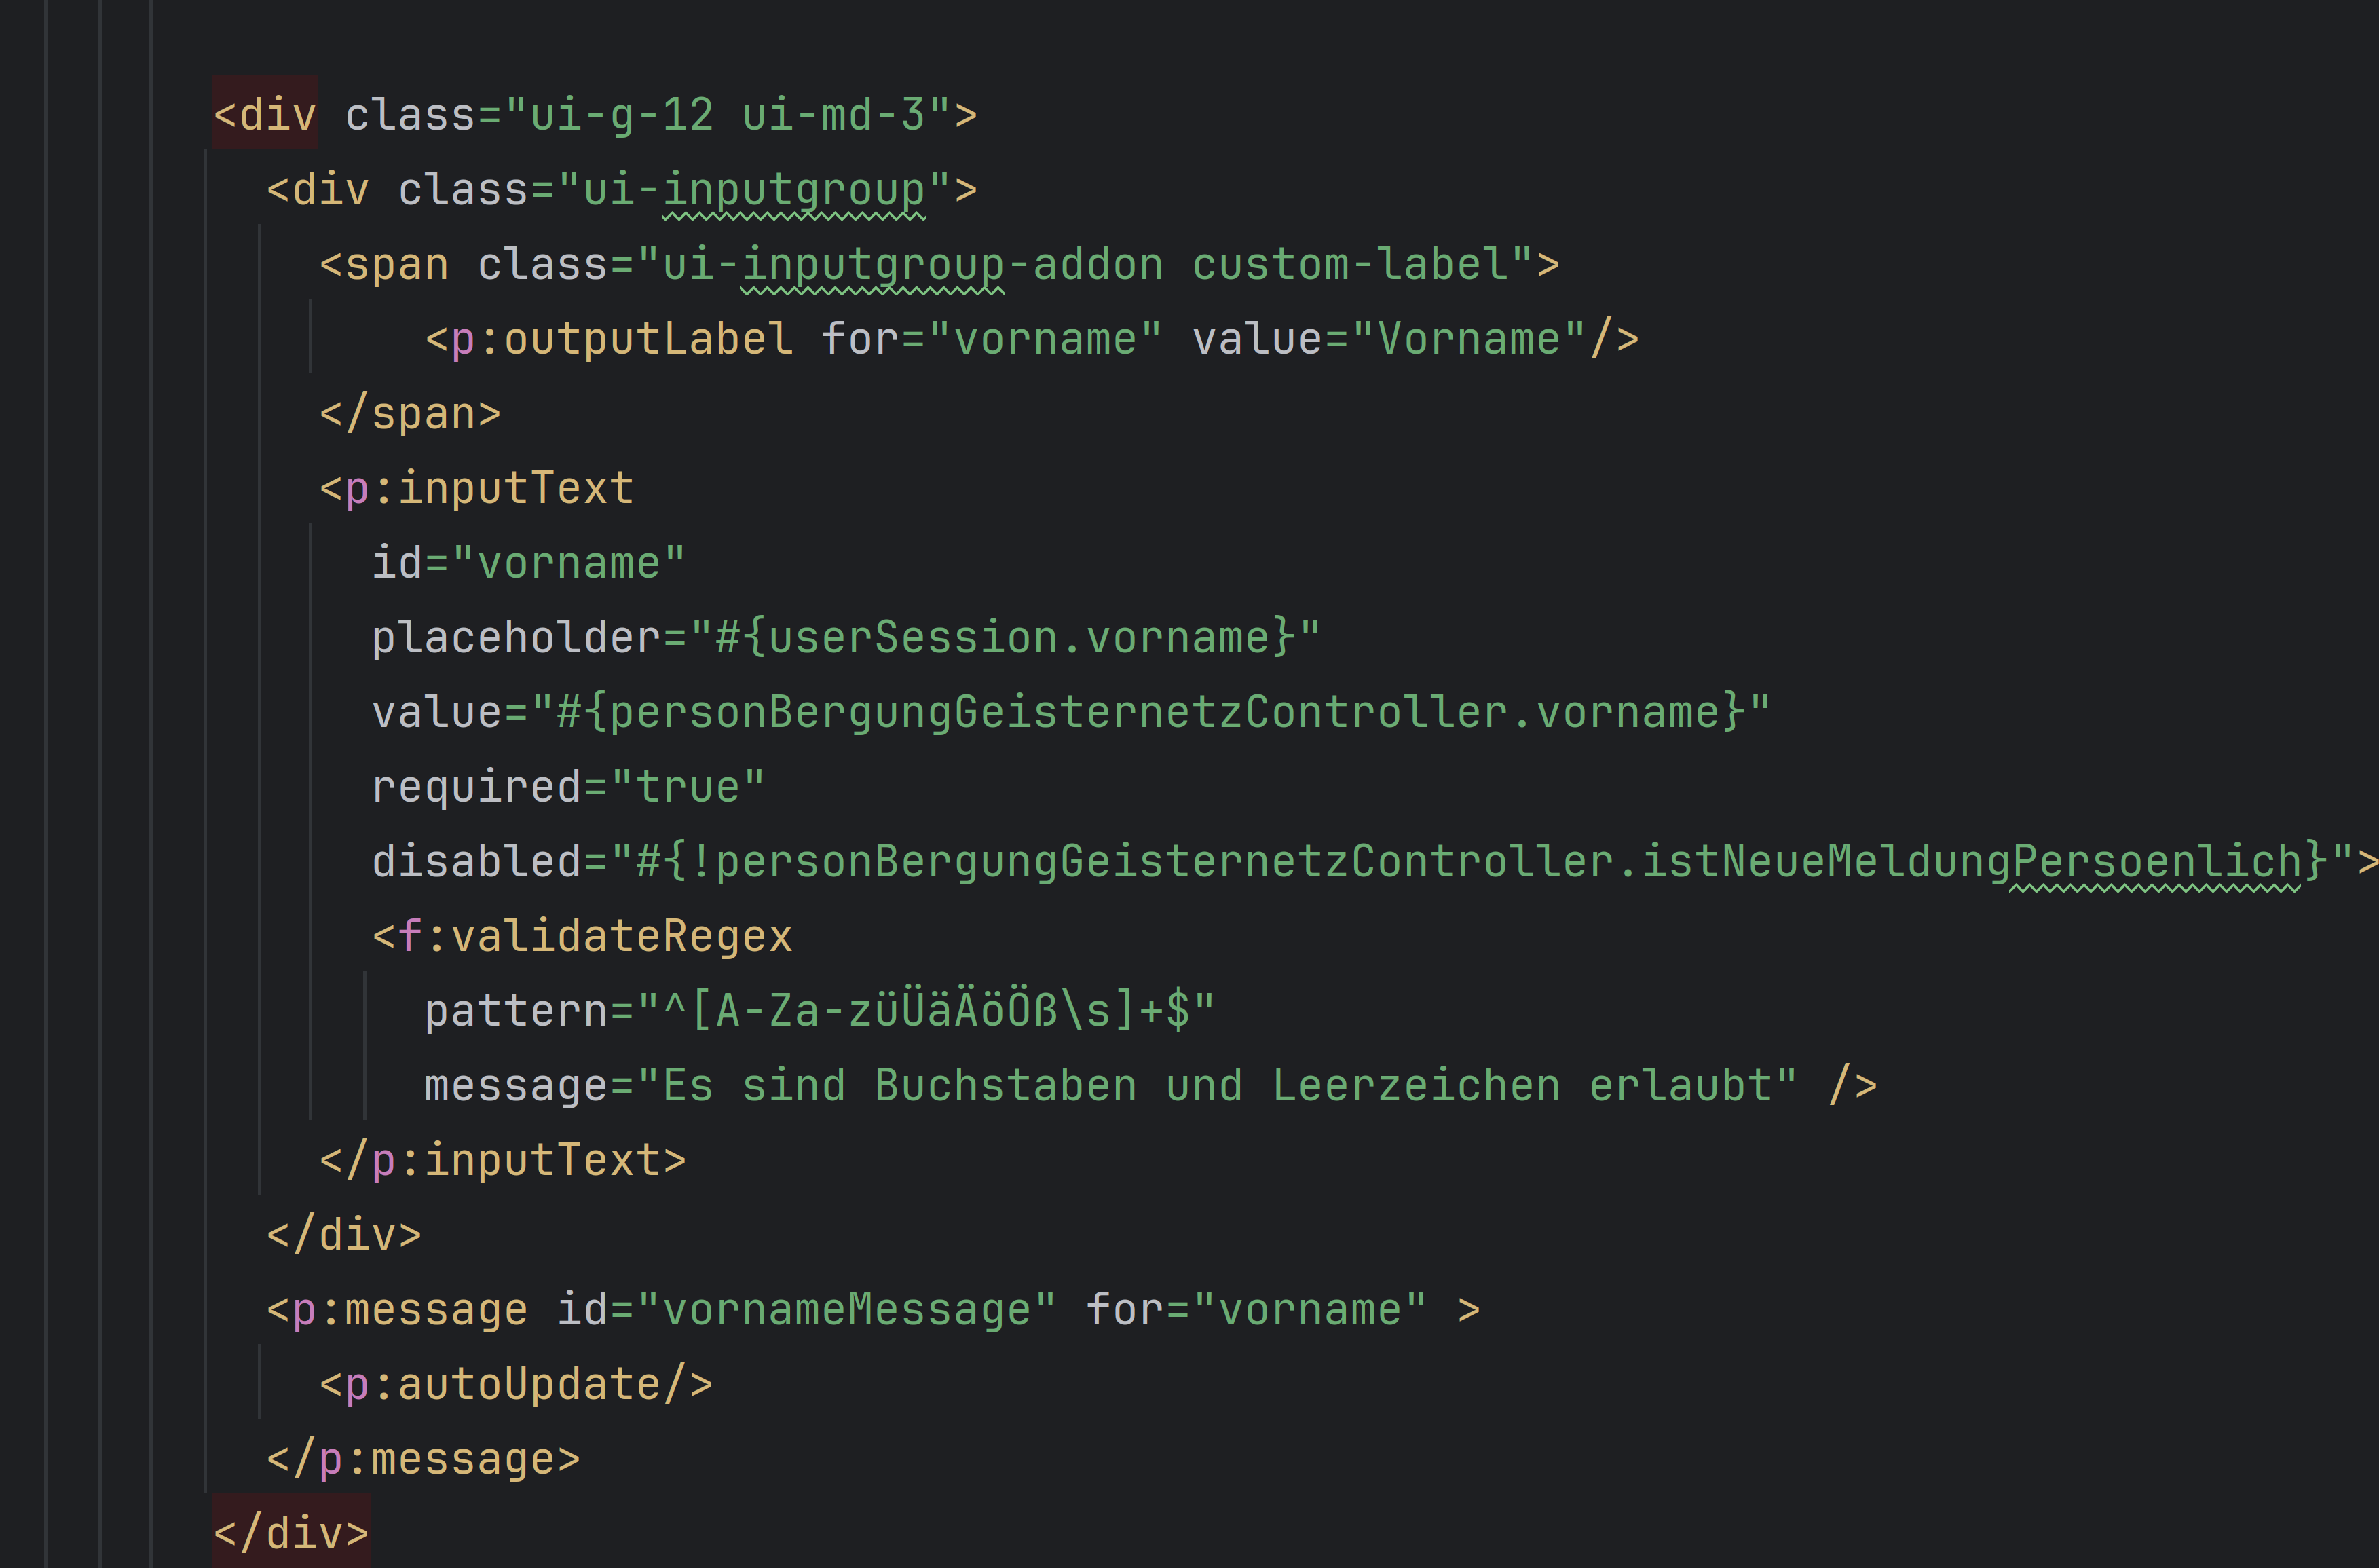
\includegraphics[width=\textwidth]{abbildungen/Verwaltungsseite-Xhtml-Formular.png}
        \caption{Verwaltungsseite Formular neue Meldung}
        \label{verwaltungsseite-formular}
    \end{figure} 

    Den ersten Bereich der Seite stellt das Formular dar. Das Formular wird von einem eindeutig indentifizierbaren h:form- und p:card-Tag ummantelt. Letzteres Tag wird mit einer individuellen Css-Klasse namens „custom-meldung-erstellen-card“ versehen, welche die Grenzlinien und den äußeren Abstand des Elements steuert.
    Da auf der Webapplikation ebenfalls das anonyme Melden von Geisternetzen gewünscht ist, wird ein p:selectBooleanButton-Tag verwendet, welcher zwischen dem persönlichen und anonymen Erfassen von Meldungen unterscheidet.
    Der Button selbst besitzt als Wert das Attribut „istNeueMeldungPersoenlich“ vom Typ „boolean“ des PersonBergungGeisternetzControllers, welcher die Sichtbarkeit personenbezogenen Felder des Formulars steuern soll.
    Um die Steuerung der Sichtbarkeit der Felder dem Endnutzer in Echtzeit zu ermöglichen, wird innerhalb des Buttons ein p:Ajax-Tag definiert. Bei jeder Änderung des Wertes wird das Formular aktualisiert.
    Der Aufbau des Formulars selbst wird über der p:inputText-Tags gesteuert. Diese stellen eine von Primefaces überarbeite Version der klassischen Eingabefelder von Html dar.
    Diese Tags werden mit dem zu steuernden Wert des PersonBergungGeisternetzControllers verknüpft. Eingabefelder, mit einem Personenbezug, werden zusätzlich mit dem Disabled-Attribut und dem Wert „!personBergungGeisternetzController.istNeueMeldungPersoenlich“ versehen.
    Letzteres Attribut steuert die Aktivierung und Deaktivierung des jeweiligen Formularfelds, in Abhängigkeit des zuvor erstellten p:selectBooleanButton-Tags.
    Innerhalb der Eingabefelder wird jeweils ein f:validateRegex-Tag hinterlegt, welcher die Nutzereingaben anhand eines \gls{regex}-Wertes steuert.
    Für das Speichern der neuen Meldung wird ein p:commandButton-Tag verwendet, der asynchron die Methode „saveNeueMeldung“ im PersonBergungGeisternetzController aufruft.  
    
    \newpage
    Die Implementierung einer Tabelle wird anhand des Beispiels von Tabelle „Offene Meldungen“ gezeigt. Klassisch wird mit dem h:form und einem folgenden p:card-Tag begonnen. Anschließend wird ein h:panelGroup-Tag zur Ummantelung der Tabelle hinterlegt und diese selbst 
    durch Verwendung des p:dataTable-Tags erstellt. Die Tabelle benötigt einen Value- und Var-Attribut, welche den gesamten Tabelleninhalt und den Wert pro Reihe steuern. Da sich diese Tabelle auf die noch offenen Meldungen von Geisternetzbergungen bezieht, wird das Value-Attribut mit der Eigenschaft „allOffeneGeisternetze“ des PersonBergungGeisternetzControllers 
    verknüpft. Das Var-Attribut mit dem Wert „offenesGeisternetz“ versehen und stellt jeden vorhanden Eintrag der adressierten Array-Liste dar.
    Die Spalten der Tabelle werden über p:column-Tags definiert, die als HeaderText-Attribut den Name der jeweiligen Spalte enthalten.
    Innerhalb der Tags wird der Spaltenwert definiert. Ist lediglich die Anzeige eines Wertes gewünscht, wird dies durch Verwendung des h:outputText-Tags umgesetzt. 
    \begin{figure}[H]
        \centering
        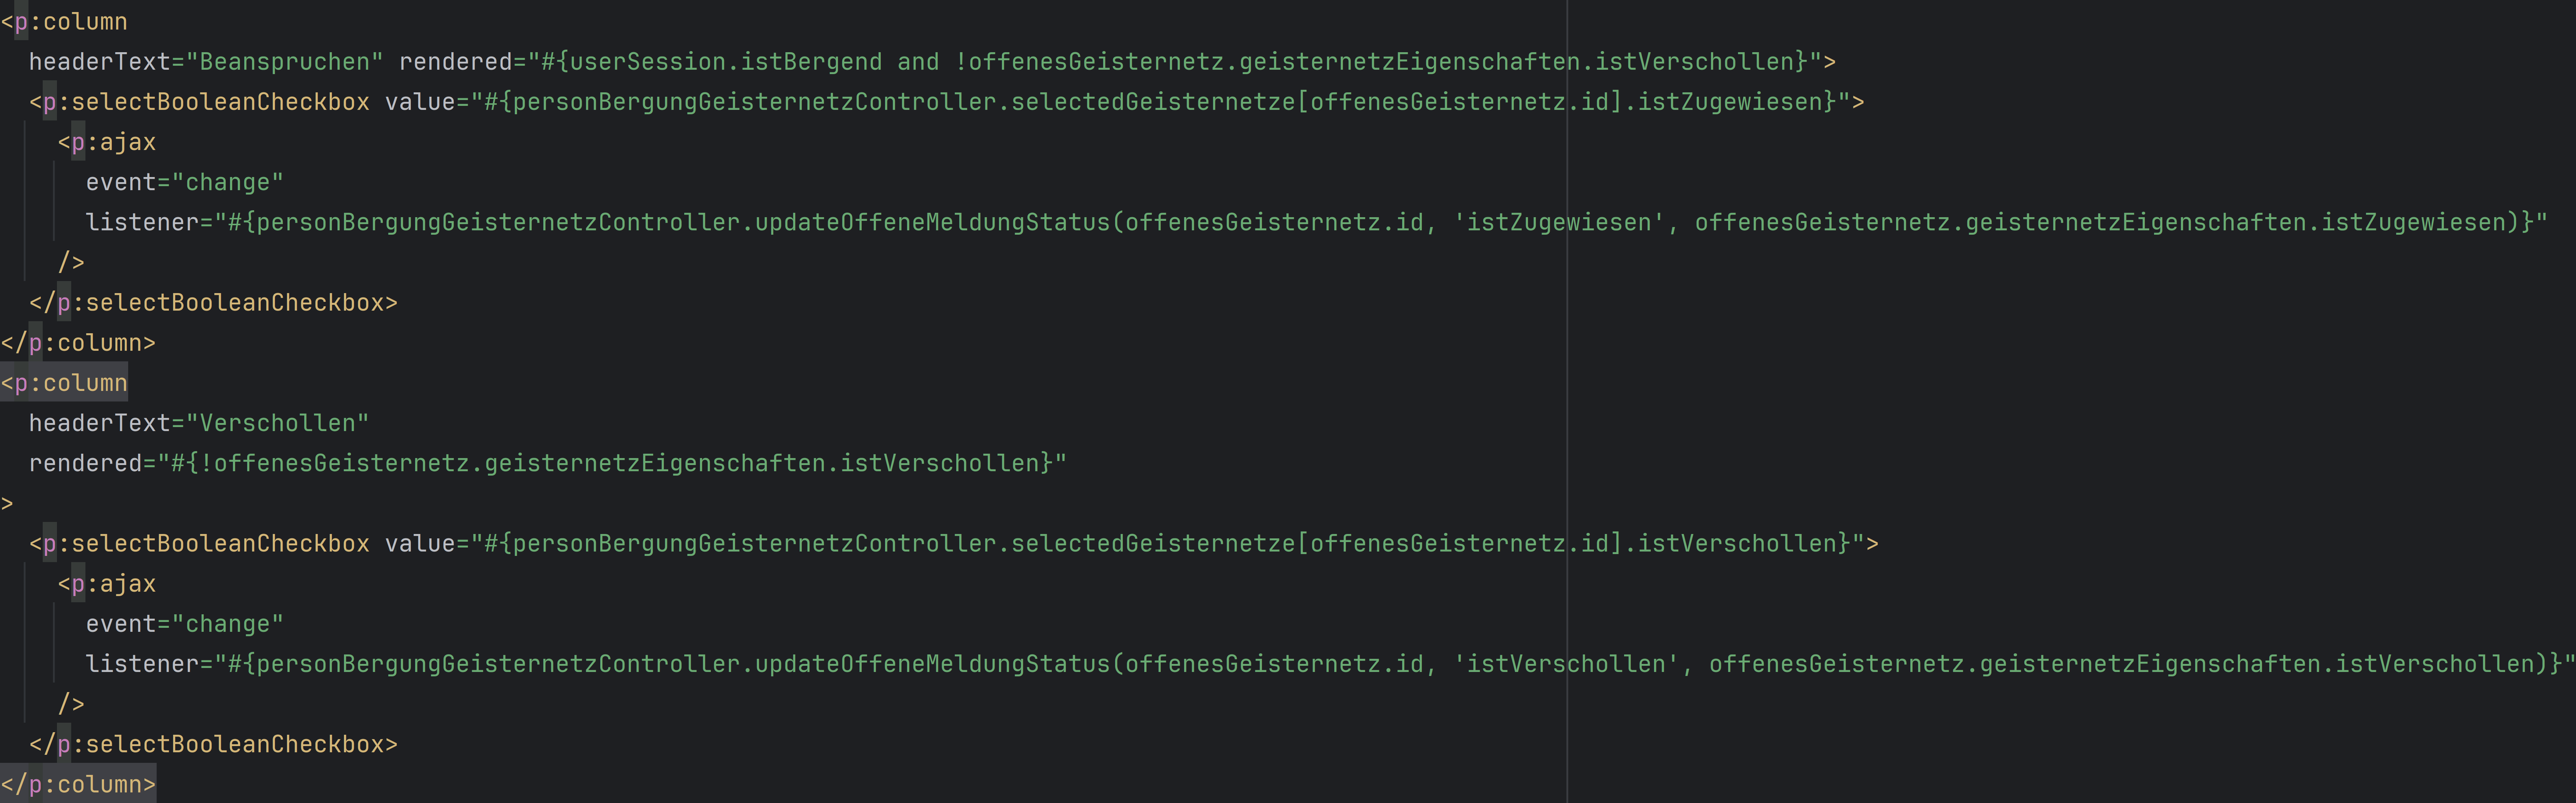
\includegraphics[width=\textwidth]{abbildungen/Verwaltungsseite-Xhtml-Offene-Bergungen.png}
        \caption{Verwaltungsseite Tabelle offene Meldungen}
        \label{verwaltungsseite-offene-meldungen}
    \end{figure} 
    Eine Besonderheit stellen die Spalten namens „Beanspruchen“ und „Verschollen“ dar, da diese eine Checkbox beinhalten, welche
    die Zuweisung eines Geisternetzes zu einer Person und das Verschollen-Melden eines Geisternetzes steuern sollen. Um diese Funktionalitäten umzusetzen, wird das p:selectBooleanCheckbox-Tag verwendet und dort als Value-Attribut die Eigenschaft „selectedGeisternetze“ der PersonBergungGeisternetzController adressiert.
    Um die Verknüpfung und Löschung der Relationen zu steuern, wir die bereits erstellte Methode „toggleGeisternetzSelection“ des PersonBergungGeisternetzControllers verwendet.
    Die Speicherung der Tabellenzustände wird durch die Methode „saveZuweisungPersonBergungGeisternetz“ des PersonBergungGeisternetzControllers gesteuert.
    
    \newpage
    \section{Testing der Webapplikation}
    Die Programmierung der Webapplikation ist beendet. Die Bereitstellung der Webapplikation ohne Testen der Anwendung birgt jedoch sowohl für den Betreiber, als auch den Endnutzer Gefahren.
    Ist beispielsweise ein Datenbankzugriff fehlerhaft, kann dieser zur Inkonsistenz von Daten führen und so das Nutzererlebnis verfälschen. Zur Fehlervermeidung wird innerhalb dieses Projekts auf Funktionstests zurückgegriffen.
    Um das klassische Verhalten eines Nutzers widerzuspiegeln, wird die Website durch zwei Testläufe auf Fehler untersucht, welche beiden auf der Login-Seite beginnen.
    
    \subsection{Fehleranalyse} 
    Der erste Testdurchlauf wird durch den Button des anonymen Logins getätigt. Nach Betätigung des Buttons wird auf die Startseite der Webapplikation weitergeleitet. Auf dieser selbst ist die Funktionalität
    einwandfrei gegebenen. Die Anzeige des Headers und der Tabellen funktioniert problemlos. Anschließend wird die Verwaltungsseite aufgerufen und eine neue persönliche und anonyme Meldung erstellt. Jede der beiden Erstellungen funktioniert fehlerfrei.
    Der erste Testdurchlauf ist somit erfolgreich abgeschlossen. Folgend ist der zweite Testdurchlauf durchzuführen. Es wird wieder auf der Loginseite der Anwendung begonnen. Während des Anwendungsfalls wird sowohl das meldende und bergende Recht an die anmeldende Testperson vergeben.
    Nach Betätigung des Anmelde-Buttons wird wie zuvor auf die Startseite der Anwendung geleitet, welche ebenfalls fehlerfrei funktioniert. Danach wird die Verwaltungsseite getestet. Das Erstellen neuer Meldungen erfolgt problemlos. Im nächsten Schritt des Testdurchlaufs gilt es die Besonderheiten, als bergende Person
    zu testen, welche sich auf das Beanspruchen und Verwalten der Geisternetzzustände bezieht. Innerhalb des Zuweisungsvorgangs tauchen Probleme auf. Das Hinzufügen und Löschen der Relationen führt zu doppelten Werten und somit Überschneidungen. 
    
    \subsection{Fehlerbehebung}
    Durch Betrachtung der Quellcodestruktur ist ersichtlich, dass der Fehler im nicht korrekten Verwalten der Listen „eingeloggtePersonZuweisungen„“ und „allOffeneGeisternetze“ liegt. Zwar wurde das Hinzufügen und Löschen der jeweiligen Liste befehligt, jedoch muss zu dessen korrekter
    Funktionalität die bestehende Methode namens „equals“ in der Geisternetz-Entität durch eine eigene Implementierung überschrieben werden, welche die Gleichheit anhand des Identifikators der Datenbank prüft. 

    \section{Retrospektive des Projektverlaufs}
    Rückblickend ist die Umsetzung des Projekts positiv verlaufen. Bei näherer Betrachtung, wurde die Struktur des Projekts und die Priorisierung der Aufgaben passend gewählt. Das Projekt konnte anhand eines roten Fadens und einer strukturierten Programmierung umgesetzt werden.
    Einen Anlass zur Verbesserung bietet die Art des Testings. Innerhalb dieses Schritts könnte das funktionale Testen durch Unit- und Integrationstests ergänzt werden, welche die Backend-Operationen gezielter untersuchen.  
    
    \newpage
    \printbibliography
    
    \end{document}
